\documentclass[12pt,spanish,]{scrartcl}
\usepackage{lmodern}
\usepackage{amssymb,amsmath}
\usepackage{ifxetex,ifluatex}
\usepackage{fixltx2e} % provides \textsubscript
\ifnum 0\ifxetex 1\fi\ifluatex 1\fi=0 % if pdftex
  \usepackage[T1]{fontenc}
  \usepackage[utf8]{inputenc}
\else % if luatex or xelatex
  \ifxetex
    \usepackage{mathspec}
  \else
    \usepackage{fontspec}
  \fi
  \defaultfontfeatures{Ligatures=TeX,Scale=MatchLowercase}
    \setmainfont[]{Ubuntu}
    \setmonofont[Mapping=tex-ansi]{Ubuntu Mono}
\fi
% use upquote if available, for straight quotes in verbatim environments
\IfFileExists{upquote.sty}{\usepackage{upquote}}{}
% use microtype if available
\IfFileExists{microtype.sty}{%
\usepackage{microtype}
\UseMicrotypeSet[protrusion]{basicmath} % disable protrusion for tt fonts
}{}
\usepackage[a4paper]{geometry}
\usepackage[unicode=true]{hyperref}
\PassOptionsToPackage{usenames,dvipsnames}{color} % color is loaded by hyperref
\hypersetup{
            colorlinks=true,
            linkcolor=Maroon,
            citecolor=Blue,
            urlcolor=Blue,
            breaklinks=true}
\urlstyle{same}  % don't use monospace font for urls
\ifnum 0\ifxetex 1\fi\ifluatex 1\fi=0 % if pdftex
  \usepackage[shorthands=off,main=spanish]{babel}
\else
  \usepackage{polyglossia}
  \setmainlanguage[]{spanish}
\fi
\usepackage{longtable,booktabs}
\usepackage{graphicx,grffile}
\makeatletter
\def\maxwidth{\ifdim\Gin@nat@width>\linewidth\linewidth\else\Gin@nat@width\fi}
\def\maxheight{\ifdim\Gin@nat@height>\textheight\textheight\else\Gin@nat@height\fi}
\makeatother
% Scale images if necessary, so that they will not overflow the page
% margins by default, and it is still possible to overwrite the defaults
% using explicit options in \includegraphics[width, height, ...]{}
\setkeys{Gin}{width=\maxwidth,height=\maxheight,keepaspectratio}
\IfFileExists{parskip.sty}{%
\usepackage{parskip}
}{% else
\setlength{\parindent}{0pt}
\setlength{\parskip}{6pt plus 2pt minus 1pt}
}
\setlength{\emergencystretch}{3em}  % prevent overfull lines
\providecommand{\tightlist}{%
  \setlength{\itemsep}{0pt}\setlength{\parskip}{0pt}}
\setcounter{secnumdepth}{5}
% Redefines (sub)paragraphs to behave more like sections
\ifx\paragraph\undefined\else
\let\oldparagraph\paragraph
\renewcommand{\paragraph}[1]{\oldparagraph{#1}\mbox{}}
\fi
\ifx\subparagraph\undefined\else
\let\oldsubparagraph\subparagraph
\renewcommand{\subparagraph}[1]{\oldsubparagraph{#1}\mbox{}}
\fi

\date{}

\begin{document}

{
\hypersetup{linkcolor=black}
\setcounter{tocdepth}{3}
\tableofcontents
}
\begin{longtable}[]{@{}l@{}}
\toprule
\begin{minipage}[t]{0.03\columnwidth}\raggedright\strut
title: Debian Post-install subtitle: Un documento de BricoLabs author: -
Sergio Alvariño
\href{mailto:salvari@gmail.com}{\nolinkurl{salvari@gmail.com}} tags:
{[}Pandoc, Documentación, makefile, git{]} date: julio-2016 lang: es-ES
abstract: \textbar{} Instalación de Debian\strut
\end{minipage}\tabularnewline
\begin{minipage}[t]{0.03\columnwidth}\raggedright\strut
Algunas notas referentes a la instalación de Debian Jessie\strut
\end{minipage}\tabularnewline
\bottomrule
\end{longtable}

\section{Introducción}\label{introducciuxf3n}

Mi portátil es un ordenador Acer 5755G con las siguientes
características:

\begin{itemize}
\item
  Core i5 2430M 2.4GHz
\item
  NVIDIA Geforce GT 540M
\item
  8Gb RAM
\item
  750Gb HD
\end{itemize}

Mi portátil equipa una tarjeta \emph{Nvidia Geforce GT540M} que resulta
pertenecer a una rama muerta en el árbol de desarrollo de Nvidia.

La gráfica es una Nvidia Optimus, es decir una tarjeta híbrida que
funcionaba perfectamente en Ubuntu 14.04 usando Bumblebee.

Con el paso a Ubuntu \emph{Xenial Xerus} mi tarjeta gráfica dejó de
funcionar correctamente con el procedimiento de instalación de Bumblebee
que venía usando. Y con todos los que fui capaz de probar.

A mayores me encontré también con problemas insalvables para instalar el
Virtual Box así que decidí volver a Debian.

Para hacer la actualización del sistema opté por desinstalar el dvd y
montar en su lugar un disco SSD en un Caddie para Acer. La instalación
fué muy fácil, y aunque el portátil arranca perfectamente de cualquiera
de los dos discos opté por instalar el SSD en la bahía del HD original y
pasar el HD al caddie.

Una vez instalado el sistema operativo, lo primero fue la instalación
del Bumblebee para probar que funcionaba normalmente.

\begin{verbatim}
sudo apt-get install firmware-linux-nonfree Bumblebee-nvidia primus
\end{verbatim}

\section{Cambiar las opciones de
idioma}\label{cambiar-las-opciones-de-idioma}

Ejecutamos:

\begin{verbatim}
sudo dpkg-reconfigure locales
\end{verbatim}

Y después solo tenemos que cambiar la selección del idioma en la
configuración de Gnome.

Nos pedirá rearrancar Gnome y renombrará todos los directorios de
sistema.

\section{Gestión de paquetes}\label{gestiuxf3n-de-paquetes}

Instalamos \emph{aptitude}, \emph{synaptic} y \emph{gdebi}

\begin{verbatim}
sudo apt-get install aptitude
sudo apt-get install synaptic
sudo apt-get install gdebi
\end{verbatim}

Cambiamos las opciones de \emph{aptitude} para que \textbf{no instale}
los paquetes recomendados.

\subsection{Quitamos el cdrom de los
sources.list}\label{quitamos-el-cdrom-de-los-sources.list}

Editamos el fichero \emph{/etc/apt/sources.list} y comentamos las lineas
del cdrom.

\subsection{Habilitamos los backports y
multimedia}\label{habilitamos-los-backports-y-multimedia}

\subsubsection{Backports:}\label{backports}

\begin{verbatim}
sudo cat > /etc/apt/sources.list.d/backports.list << EOF
# backports
deb http://ftp.debian.org/debian/ jessie-backports main contrib non-free
EOF
\end{verbatim}

\subsubsection{Multimedia:}\label{multimedia}

\begin{verbatim}
sudo cat >> /etc/apt/sources.list.d/multimedia.list << EOF
# multimedia
deb http://www.deb-multimedia.org/ jessie main non-free
EOF

sudo apt-get -y --allow-unauthenticated install --reinstall deb-multimedia-keyring
\end{verbatim}

Y actualizamos

\begin{verbatim}
sudo aptitude update
\end{verbatim}

\section{Instalación de varios paquetes
sueltos}\label{instalaciuxf3n-de-varios-paquetes-sueltos}

\subsection{Programas de utilidad y uso
frecuente}\label{programas-de-utilidad-y-uso-frecuente}

\subsubsection{Menulibre}\label{menulibre}

Un editor de menús para Gnome, nos permite generar los archivos desktop
para cualquier aplicación. Mucho más completo que \emph{alacarte} la
otra alternativa.

\begin{verbatim}
sudo apt-get install menulibre
\end{verbatim}

\subsubsection{Terminator}\label{terminator}

Terminator es un emulador de terminal muy completo y muy flexible. Los
instalamos desde \emph{aptitude}

\begin{verbatim}
sudo aptitude install terminator python-keybinder
\end{verbatim}

\subsubsection{Keepass2}\label{keepass2}

Instalado \emph{keepass2} desde Debian

\begin{verbatim}
sudo aptitude install keepass2
\end{verbatim}

\subsubsection{gksu}\label{gksu}

Un \emph{sudo} en modo gráfico:

\begin{verbatim}
sudo aptitude install gksu
\end{verbatim}

\textbf{Muy importante} ejecutar \texttt{gksu-properties} y escoger el
modo \texttt{sudo} en lugar de \texttt{su}. Nos evitaremos problemas con
la instalación de muchas aplicaciones.

\subsubsection{Diskmanager}\label{diskmanager}

Para gestionar discos portátiles

\begin{verbatim}
sudo apt-get install ntfs-3g disk-manager
\end{verbatim}

\subsubsection{Gnucash}\label{gnucash}

Finanzas en linux, para mi imprescindible.

\begin{verbatim}
sudo apt-get -t jessie-backports install gnucash
\end{verbatim}

\subsubsection{\texorpdfstring{Herramientas
\emph{sync}}{Herramientas sync}}\label{herramientas-sync}

La uso para hacer mis backups a discos externos.

\begin{verbatim}
sudo apt-get install rsync grsync
\end{verbatim}

\subsubsection{Dropbox}\label{dropbox}

Bajado el paquete Debian desde la página
\href{https://www.dropbox.com/install-linux}{web de Dropbox}, instalado
el paquete con \emph{packageinstall}, es decir, simplemente pinchando
desde el gestor de ficheros.

\subsubsection{Compresores et al}\label{compresores-et-al}

\begin{verbatim}
sudo apt-get install rar unrar zip unzip unace bzip2 lzop p7zip p7zip-full p7zip-rar
\end{verbatim}

\subsubsection{Freeplane}\label{freeplane}

Mejor que
\href{http://freemind.sourceforge.net/wiki/index.php/Main_Page}{Freemind}
(en mi opinión). El baile de siempre, descargar de la
\href{http://www.freeplane.org/}{web}, descomprimir en
\emph{\textasciitilde{}/apps} y crear lanzador con \emph{MenuLibre}.
Todos los ficheros que tenía de \emph{Freemind} se pueden usar
directamente con \emph{Freeplane}.

\subsubsection{Telegram desktop}\label{telegram-desktop}

El cliente de mensajeria de Telegram. Descargado desde la web, instalado
en \emph{\textasciitilde{}/apps}

\subsection{Internet}\label{internet}

\subsubsection{Chrome y Chromium}\label{chrome-y-chromium}

Instalado chrome añadiendo fuentes a aptitude. No recuerdo como las
añadí, pero en el fichero
\emph{/etc/apt/sources.list.d/google-chrome.list}, tengo los siguientes
contenidos:

\begin{verbatim}
###
###
###
###
### THIS FILE IS AUTOMATICALLY CONFIGURED ###
# You may comment out this entry, but any other modifications may be lost.
deb [arch=amd64] http://dl.google.com/linux/chrome/deb/ stable main
\end{verbatim}

Ejecutamos:

\begin{verbatim}
sudo aptitude install google-chrome-stable
sudo aptitude install chromium
\end{verbatim}

\subsubsection{Tor}\label{tor}

El navegador anónimo.

Bajamos el zip de la aplicación desde la
\href{https://www.torproject.org}{web} y descomprimido en
\emph{\textasciitilde{}/apps} copiado el fichero desktop a
\emph{\textasciitilde{}/.local/share/applications}

\subsubsection{openvpn}\label{openvpn}

Basado en la web
\href{https://nixbsd.wordpress.com/2017/04/01/freebsd-10-2-configure-openvpn-client/}{nix/bsd}.

\subsubsection{Deluge}\label{deluge}

El cliente torrent que uso habitualmente. Instalamos desde aptitude

\begin{verbatim}
sudo aptitude install deluge
xdg-mime default deluge.desktop x-scheme-handler/magnet
\end{verbatim}

\subsubsection{TiddlyDesktop}\label{tiddlydesktop}

\emph{Tiddly} es una wiki auto-contenida y muy flexible, tiene un sinfin
de versiones adaptadas para diferentes usos. Hace años que la uso como
cuaderno de bitácora personal, pero no había seguido su evolución.

Me he descargado:

\begin{itemize}
\tightlist
\item
  \href{http://tiddlywiki.com/}{Tiddlywiki} y le he instalado los
  plugins de \emph{FontAwesome} y \emph{WikiMap}, este será mi nuevo
  cuaderno de bitácora.
\item
  \href{http://gsd5.tiddlyspot.com/}{GSD5} un \emph{TiddlyWiki} adaptado
  a \emph{GTD}
\end{itemize}

A mayores me he instalado la aplicación
\href{https://github.com/Jermolene/TiddlyDesktop}{TiddlyDesktop}, basada
en \emph{node webkit} que simplifica el tema de backups (en teoría).

Como siempre la instalamos en \emph{\textasciitilde{}/apps} y creamos un
lanzador con \emph{MenuLibre}.

\subsection{Gráficos}\label{gruxe1ficos}

\subsubsection{Inkscape}\label{inkscape}

El programa libre para creación y edición de gráficos vectoriales.

\begin{verbatim}
apt-cache policy inkscape
apt-get -t jessie-backports install inkscape
aptitude install ink-generator
\end{verbatim}

\subsubsection{LibreCAD y FreeCAD}\label{librecad-y-freecad}

Imprescindibles para el diseño de cacharros. Instalados desde repos con
aptitude

\begin{verbatim}
apt-get install librecad

apt-get -t jessie-backports install freecad
\end{verbatim}

\subsubsection{Gimp}\label{gimp}

El programa para edición y retocado de imágenes.

Gimp ya estaba instalado, adicionalmente instalado el gimp data-extra

\begin{verbatim}
sudo aptitude install gimp-plugin-registry gimp-texturize gimp-data-extras gimp-gap
\end{verbatim}

\subsubsection{Shutter}\label{shutter}

Un programa de captura de pantallas que permite editarlas rápida y
fácilmente:

\begin{verbatim}
sudo aptitude install shutter libgoo-canvas-perl
\end{verbatim}

\subsubsection{Pencil}\label{pencil}

Una aplicación java para hacer esquemas de aplicaciones web, puede que
no lo necesites.

Descargar la última versión (paquete Debian) desde
\href{http://pencil.evolus.vn/}{la página web}. Lo instalamos y listo.
Puede dar problemas si usamos Iceweasel, ya que el paquete depende de
Firefox. Más info
\href{https://www.linuxwebzone.com/install-pencil-on-debian/}{aquí}

\subsection{Fotografía}\label{fotografuxeda}

\subsubsection{Rawtherapee y Darktable: Tratamiento de imágenes
fotogŕaficas}\label{rawtherapee-y-darktable-tratamiento-de-imuxe1genes-fotogux155aficas}

Si te gusta la fotografía y/o tienes una cámara reflex, definitivamente
necesitas estas aplicaciones.

\begin{verbatim}
sudo aptitude install icc-profiles icc-profiles-free
sudo aptitude install rawtherapee darktable
\end{verbatim}

\subsubsection{Stopmotion}\label{stopmotion}

Para hacer pélis de animación Stopmotion.

\begin{verbatim}
sudo aptitude install stopmotion vgrabbj dvgrab
\end{verbatim}

TODO: Probar qStopmotion

\subsection{Audio y video}\label{audio-y-video}

\subsubsection{Codecs}\label{codecs}

Instalamos los codecs

\begin{verbatim}
sudo apt-get install libav-tools

sudo apt-get install faad gstreamer0.10-ffmpeg gstreamer0.10-x \
gstreamer0.10-fluendo-mp3 gstreamer0.10-plugins-base \
gstreamer0.10-plugins-good gstreamer0.10-plugins-bad \
gstreamer0.10-plugins-ugly ffmpeg lame twolame vorbis-tools \
libquicktime2 libfaac0 libmp3lame0 libxine2-all-plugins libdvdread4 \
libdvdnav4 libmad0 sox libxvidcore4 libstdc++5

sudo apt-get install w64codecs
\end{verbatim}

\subsubsection{Reproductores de
música}\label{reproductores-de-muxfasica}

Instalamos \emph{Clementine}, \emph{decibel}, \emph{audacity},
\emph{soundconverter}:

\begin{verbatim}
sudo aptitude install clementine gstreamer0.10-plugins-bad
sudo aptitude install decibel-audio-player audacity soundconverter
\end{verbatim}

\subsubsection{Gpodder}\label{gpodder}

Instalamos \emph{gpodder} para gestionar nuestros podcast, aunque
\emph{Clementine} también nos vale.

\begin{verbatim}
sudo aptitude install gpodder
\end{verbatim}

\subsubsection{Spotify}\label{spotify}

Cliente de \emph{Spotify}

\begin{verbatim}
sudo apt-key adv --keyserver hkp://keyserver.ubuntu.com:80 --recv-keys BBEBDCB318AD50EC6865090613B00F1FD2C19886
echo deb http://repository.spotify.com stable non-free | sudo tee /etc/apt/sources.list.d/spotify.list
sudo aptitude update
sudo aptitude install spotify-client
\end{verbatim}

\subsubsection{Video}\label{video}

Instalamos también utilidades de video:

\begin{verbatim}
sudo aptitude install vlc browser-plugin-vlc
sudo aptitude install recordmydesktop gtk-recordmydesktop
sudo aptitude install vokoscreen
sudo aptitude install handbrake handbrake-cli handbrake-gtk
\end{verbatim}

\subsection{Seguridad}\label{seguridad}

\subsubsection{Lector de DNIe}\label{lector-de-dnie}

Instalamos:

\begin{verbatim}
sudo aptitude libccid install pcscd pcsc-tools
\end{verbatim}

Como root ejecutamos \emph{pcsc\_scan} \footnote{Es posible que sean
  necesario reiniciar el pc antes de seguir}:

\begin{verbatim}
root@rasalhague:~# pcsc_scan 
PC/SC device scanner
V 1.4.23 (c) 2001-2011, Ludovic Rousseau <ludovic.rousseau@free.fr>
Compiled with PC/SC lite version: 1.8.11
Using reader plug'n play mechanism
Scanning present readers...
Waiting for the first reader...
\end{verbatim}

Si insertamos el lector veremos algo como esto:

\begin{verbatim}
root@rasalhague:~# pcsc_scan 
PC/SC device scanner
V 1.4.23 (c) 2001-2011, Ludovic Rousseau <ludovic.rousseau@free.fr>
Compiled with PC/SC lite version: 1.8.11
Using reader plug'n play mechanism
Scanning present readers...
Waiting for the first reader...found one
Scanning present readers...
0: C3PO LTC31 v2 (11061005) 00 00

Wed Jan 25 01:17:20 2017
Reader 0: C3PO LTC31 v2 (11061005) 00 00
  Card state: Card removed, 
\end{verbatim}

Si insertamos un DNI veremos que se lee la información de la tarjeta
insertada:

\begin{verbatim}
Reader 0: C3PO LTC31 v2 (11061005) 00 00
  Card state: Card inserted, 
y mas rollo
\end{verbatim}

Instalamos ahora:

\begin{verbatim}
aptitude install pinentry-gtk2 opensc
\end{verbatim}

\section{Documentos}\label{documentos}

\subsection{Calibre}\label{calibre}

La mejor utilidad para gestionar tu colección de libros electrónicos.

Ejecutamos lo que manda la página web:

\begin{verbatim}
sudo -v && wget -nv -O- https://raw.githubusercontent.com/kovidgoyal/calibre/master/setup/linux-installer.py \
| sudo python -c "import sys; main=lambda:sys.stderr.write('Download failed\n'); exec(sys.stdin.read()); main()"
\end{verbatim}

Para usar el calibre con el Kobo Glo:

\begin{itemize}
\item
  Desactivamos todos los plugin de Kobo menos el \emph{Kobo Touch
  Extended}
\item
  Creamos una columna \emph{MyShelves} con identificativo
  \emph{\#myshelves}
\item
  En las opciones del plugin:

  \begin{itemize}
  \tightlist
  \item
    En la opción \emph{Collection columns} añadimos las columnas
    \emph{series,\#myshelves}
  \item
    Marcamos las opciones \emph{Create collections} y \emph{Delete empy
    collections}
  \item
    \emph{Update metadata on device} y \emph{Set series information}
  \end{itemize}
\end{itemize}

Algunos enlaces útiles:

\begin{itemize}
\tightlist
\item
  \url{https://github.com/jgoguen/calibre-kobo-driver}
\item
  \url{http://www.lectoreselectronicos.com/foro/showthread.php?15116-Manual-de-instalaci\%C3\%B3n-y-uso-del-plugin-Kobo-Touch-Extended-para-Calibre}
\item
  \url{http://www.redelijkheid.com/blog/2013/7/25/kobo-glo-ebook-library-management-with-calibre}
\item
  \url{https://www.netogram.com/kobo.htm}
\end{itemize}

\subsection{Pandoc}\label{pandoc}

Pandoc es un traductor entre formatos de documento. Está escrito en
Python y es increiblemente útil. De hecho este documento está escrito
con \emph{Pandoc}.

Instalado el Pandoc descargando paquete \emph{deb} desde la página web
del Pandoc.

Descargamos las plantillas desde
\href{https://github.com/jgm/pandoc-templates}{el repo} ejecutando los
siguientes comandos:

\begin{verbatim}
cd ~/.pandoc
git clone https://github.com/jgm/pandoc-templates templates
\end{verbatim}

\subsection{Zotero}\label{zotero}

Zotero es un programa que te permite guardar una o varias bibliografías
con referencias a libros, páginas web o documentos electrónicos.

Instalado el Zotero Standalone desde la
\href{https://www.zotero.org/}{página web del programa}

\subsection{Vanilla LaTeX}\label{vanilla-latex}

El LaTeX de Debian está un poquillo anticuado, si se quiere usar una
versión reciente hay que aplicar
\href{http://tex.stackexchange.com/questions/1092/how-to-install-vanilla-texlive-on-debian-or-ubuntu}{este
truco}.

\begin{verbatim}
cd ~
mkdir tmp
cd tmp
wget http://mirror.ctan.org/systems/texlive/tlnet/install-tl-unx.tar.gz
tar xzf install-tl-unx.tar.gz
cd install-tl-xxxxxx
\end{verbatim}

La parte xxxxxx varía en función del estado de la última versión de
LaTeX disponible.

\begin{verbatim}
sudo ./install-tl
\end{verbatim}

Una vez lanzada la instalación podemos desmarcar las opciones que
instalan la documentación y las fuentes. Eso nos obligará a consultar la
documentación \emph{on line} pero ahorrará practicamente el 50\% del
espacio necesario. En mi caso sin \emph{doc} ni \emph{src} ocupa 2,3Gb

\begin{verbatim}
mkdir -p /opt
sudo ln -s /usr/local/texlive/2016/bin/* /opt/texbin
\end{verbatim}

Por último para acabar la instalación añadimos \textbf{/opt/texbin} al
\emph{path}.

\subsubsection{Falsificando paquetes}\label{falsificando-paquetes}

Ya tenemos el \textbf{texlive} instalado, ahora necesitamos que el
gestor de paquetes sepa que ya lo tenemos instalado.

\begin{verbatim}
sudo apt-get install equivs --no-install-recommends
mkdir -p /tmp/tl-equivs && cd /tmp/tl-equivs
equivs-control texlive-local
\end{verbatim}

Para hacerlo más fácil podemos descargarnos un fichero ya preparado,
ejecutando:

\begin{verbatim}
wget http://www.tug.org/texlive/files/debian-equivs-2015-ex.txt
/bin/cp -f debian-equivs-2015-ex.txt texlive-local
\end{verbatim}

Editamos la versión y

\begin{verbatim}
equivs-build texlive-local
sudo dpkg -i texlive-local_2015-1_all.deb
\end{verbatim}

Todo listo, ahora podemos instalar cualquier paquete que dependa de
texlive

\subsubsection{Fuentes}\label{fuentes}

Para dejar disponibles las fuentes opentype y truetype que vienen con
texlive para el resto de aplicaciones:

\begin{verbatim}
sudo cp $(kpsewhich -var-value TEXMFSYSVAR)/fonts/conf/texlive-fontconfig.conf /etc/fonts/conf.d/09-texlive.conf
gksudo gedit /etc/fonts/conf.d/09-texlive.conf
\end{verbatim}

Borramos la linea:

\begin{verbatim}
<dir>/usr/local/texlive/2016/texmf-dist/fonts/type1</dir>
\end{verbatim}

Y ejecutamos:

\begin{verbatim}
sudo fc-cache -fsv
\end{verbatim}

\subsubsection{Actualizaciones}\label{actualizaciones}

Para actualizar nuestro latex a la última versión de todos los paquetes:

\begin{verbatim}
sudo /opt/texbin/tlmgr update --self
sudo /opt/texbin/tlmgr update --all
\end{verbatim}

También podemos lanzar el instalador gráfico con:

\begin{verbatim}
sudo /opt/texbin/tlmgr --gui
\end{verbatim}

Para usar el instalador gráfico hay que instalar previamente:

\begin{verbatim}
sudo apt-get install perl-tk --no-install-recommends
\end{verbatim}

\subsubsection{Lanzador para el actualizador de
texlive}\label{lanzador-para-el-actualizador-de-texlive}

\begin{verbatim}
mkdir -p ~/.local/share/applications
/bin/rm ~/.local/share/applications/tlmgr.desktop
cat > ~/.local/share/applications/tlmgr.desktop << EOF
[Desktop Entry]
Version=1.0
Name=TeX Live Manager
Comment=Manage TeX Live packages
GenericName=Package Manager
Exec=gksu -d -S -D "TeX Live Manager" '/opt/texbin/tlmgr -gui'
Terminal=false
Type=Application
Icon=system-software-update
EOF
\end{verbatim}

Ojo que hay que dejar instalado el gksu (aunque debería estar de antes
si sigues este doc)

\begin{verbatim}
sudo aptitude install gksu
\end{verbatim}

\subsection{Emacs}\label{emacs}

Instalado emacs desde los repos:

\begin{verbatim}
sudo aptitude install emacs
\end{verbatim}

Instalamos los paquetes \emph{markdown-mode}, \emph{mardown-plus} y
\emph{pandoc-mode} desde el menú de gestión de paquetes de
\textbf{emacs}.

También instalamos \emph{d-mode} y \emph{flymake-d}.

Después de probar \emph{flymake} y \emph{flycheck} al final me ha
gustado más \emph{flycheck} Hay una sección de configuración en el
fichero \emph{.emacs} para cada uno de ellos, pero la de \emph{flymake}
está comentada.

Configuramos el fichero \emph{.emacs} definimos algunas preferencias,
algunas funciones útiles y añadimos orígenes extra de paquetes.

\begin{verbatim}
(custom-set-variables
 ;; custom-set-variables was added by Custom.
 ;; If you edit it by hand, you could mess it up, so be careful.
 ;; Your init file should contain only one such instance.
 ;; If there is more than one, they won't work right.
 '(show-paren-mode t))
(custom-set-faces
 ;; custom-set-faces was added by Custom.
 ;; If you edit it by hand, you could mess it up, so be careful.
 ;; Your init file should contain only one such instance.
 ;; If there is more than one, they won't work right.
 )

;;------------------------------------------------------------
;; Some settings
(setq inhibit-startup-message t) ; Eliminate FSF startup msg
(setq frame-title-format "%b")   ; Put filename in titlebar
;(setq visible-bell t)            ; Flash instead of beep
(set-scroll-bar-mode 'right)     ; Scrollbar placement
(show-paren-mode t)              ; Blinking cursor shows matching parentheses
(setq column-number-mode t)  ; Show column number of current cursor location
(mouse-wheel-mode t)         ; wheel-mouse support

(setq fill-column 78)
(setq auto-fill-mode t)          ; Set line width to 78 columns...

(setq-default indent-tabs-mode nil)       ; Insert spaces instead of tabs
(global-set-key "\r" 'newline-and-indent) ; turn autoindenting on
;(set-default 'truncate-lines t)           ; Truncate lines for all buffers
;(require 'iso-transl)                     ; doesn't seems to be needed in debian


;;------------------------------------------------------------
;; Some useful key definitions
(define-key global-map [M-S-down-mouse-3] 'imenu)
(global-set-key [C-tab] 'hippie-expand)                    ; expand
(global-set-key [C-kp-subtract] 'undo)                     ; [Undo] 
(global-set-key [C-kp-multiply] 'goto-line)                ; goto line
(global-set-key [C-kp-add] 'toggle-truncate-lines)         ; goto line
(global-set-key [C-kp-divide] 'delete-trailing-whitespace) ; delete trailing whitespace
(global-set-key [C-kp-decimal] 'completion-at-point)       ; complete at point
(global-set-key [C-M-prior] 'next-buffer)                  ; next-buffer
(global-set-key [C-M-next] 'previous-buffer)               ; previous-buffer

;;------------------------------------------------------------
;; Set encoding
(prefer-coding-system 'utf-8)
(setq coding-system-for-read 'utf-8)
(setq coding-system-for-write 'utf-8)

;;------------------------------------------------------------
;; Maximum colors
(cond ((fboundp 'global-font-lock-mode)  ; Turn on font-lock (syntax highlighting)
       (global-font-lock-mode t)               ; in all modes that support it
       (setq font-lock-maximum-decoration t))) ; Maximum colors

;;------------------------------------------------------------
;; Use % to match various kinds of brackets...
;; See: http://www.lifl.fr/~hodique/uploads/Perso/patches.el

(global-set-key "%" 'match-paren)               ; % key match parents
(defun match-paren (arg)
  "Go to the matching paren if on a paren; otherwise insert %."
  (interactive "p")
  (let ((prev-char (char-to-string (preceding-char)))
        (next-char (char-to-string (following-char))))
    (cond ((string-match "[[{(<]" next-char) (forward-sexp 1))
          ((string-match "[\]})>]" prev-char) (backward-sexp 1))
          (t (self-insert-command (or arg 1))))))

;;------------------------------------------------------------
;; The wonderful bubble-buffer
(defvar LIMIT 1)
(defvar time 0)
(defvar mylist nil)

(defun time-now ()
   (car (cdr (current-time))))

(defun bubble-buffer ()
   (interactive)
   (if (or (> (- (time-now) time) LIMIT) (null mylist))
       (progn (setq mylist (copy-alist (buffer-list)))
          (delq (get-buffer " *Minibuf-0*") mylist)
          (delq (get-buffer " *Minibuf-1*") mylist)))
   (bury-buffer (car mylist))
   (setq mylist (cdr mylist))
   (setq newtop (car mylist))
   (switch-to-buffer (car mylist))
   (setq rest (cdr (copy-alist mylist)))
   (while rest
     (bury-buffer (car rest))
     (setq rest (cdr rest)))
   (setq time (time-now))) 

(global-set-key [f8] 'bubble-buffer)    ; win-tab switch the buffer

(defun geosoft-kill-buffer ()
   ;; Kill default buffer without the extra emacs questions
   (interactive)
   (kill-buffer (buffer-name))
   (set-name)) 
(global-set-key [C-delete] 'geosoft-kill-buffer) 

;;----------------------------------------------------------------------
;; MELPA and others
(when (>= emacs-major-version 24)
  (require 'package)
  (package-initialize)
  (add-to-list 'package-archives '("melpa" . "http://melpa.org/packages/") t)
  (add-to-list 'package-archives '("gnu" . "http://elpa.gnu.org/packages/") t)
  (add-to-list 'package-archives '("marmalade" . "https://marmalade-repo.org/packages/") t)
  )

; (add-to-list 'load-path "~/.emacs.d/")

;;----------------------------------------------------------------------
;; Packages installed via package
;;------------------------------

;;----------------------------------------------------------------------
;; flymake and flycheck installed from package
;; I think you have to choose only one

;; (require 'flymake)
;; ;;(global-set-key (kbd "C-c d") 'flymake-display-err-menu-for-current-line)
;; (global-set-key (kbd "C-c d") 'flymake-popup-current-error-menu)
;; (global-set-key (kbd "C-c n") 'flymake-goto-next-error)
;; (global-set-key (kbd "C-c p") 'flymake-goto-prev-error)

(add-hook 'after-init-hook #'global-flycheck-mode)
(global-set-key  (kbd "C-c C-p") 'flycheck-previous-error)
(global-set-key  (kbd "C-c C-n") 'flycheck-next-error)

;; Define d-mode addons
;; Activate flymake or flycheck for D
;; Activate auto-complete-mode
;; Activate yasnippet minor mode if available
;; Activate dcd-server
(require 'ac-dcd)
(add-hook 'd-mode-hook
          (lambda()
            ;;(flymake-d-load)
            (flycheck-dmd-dub-set-variables)
            (require 'flycheck-d-unittest)
            (setup-flycheck-d-unittest)
            (auto-complete-mode t)
            (when (featurep 'yasnippet)
              (yas-minor-mode-on))
            (ac-dcd-maybe-start-server)
            (ac-dcd-add-imports)
            (add-to-list 'ac-sources 'ac-source-dcd)
            (define-key d-mode-map (kbd "C-c ?") 'ac-dcd-show-ddoc-with-buffer)
            (define-key d-mode-map (kbd "C-c .") 'ac-dcd-goto-definition)
            (define-key d-mode-map (kbd "C-c ,") 'ac-dcd-goto-def-pop-marker)
            (define-key d-mode-map (kbd "C-c s") 'ac-dcd-search-symbol)
            (when (featurep 'popwin)
              (add-to-list 'popwin:special-display-config
                           `(,ac-dcd-error-buffer-name :noselect t))
              (add-to-list 'popwin:special-display-config
                           `(,ac-dcd-document-buffer-name :position right :width 80))
              (add-to-list 'popwin:special-display-config
                           `(,ac-dcd-search-symbol-buffer-name :position bottom :width 5)))))

;; Define diet template mode (this is not installed from package)
(add-to-list 'auto-mode-alist '("\\.dt$" . whitespace-mode))
(add-hook 'whitespace-mode-hook
          (lambda()
            (setq tab-width 2)
            (setq whitespace-line-column 250)
            (setq indent-tabs-mode nil)
            (setq indent-line-function 'insert-tab)))

;;----------------------------------------------------------------------
;; elpy
(elpy-enable)
\end{verbatim}

\subsection{Textadept}\label{textadept}

Un potente editor de desarrollo, multiplataforma.

Viene incluido en el pack D-apt, por que es muy potente como IDE para
\textbf{D}.

De momento lo único que he configurado es la fuente, para ello editamos
el fichero \emph{\textasciitilde{}/.textadept/init.lua} y añadimos la
linea:

\begin{verbatim}
ui.set_theme('light', {font = 'Meslo LG L Regular for Powerline', fontsize = 14})
\end{verbatim}

\subsection{Scribus}\label{scribus}

Scribus es un programa libre de composición de documentos. con Scribus
puedes elaborar desde los folletos de una exposición hasta una revista o
un poster.

Instalado con aptitude

\begin{verbatim}
sudo aptitude install scribus
\end{verbatim}

\subsection{Comix}\label{comix}

Mi lector de comics favorito.

Instalado con aptitude

\begin{verbatim}
sudo aptitude install comix
\end{verbatim}

\section{Desarrollo sw}\label{desarrollo-sw}

\subsection{Paquetes esenciales}\label{paquetes-esenciales}

Estos son los paquetes esenciales para empezar a desarrollar software en
Linux.

\begin{verbatim}
sudo apt-get install build-essential checkinstall make automake cmake autoconf git git-core dpkg wget
\end{verbatim}

\subsection{Git}\label{git}

Control de versiones distribuido. Imprescindible.

Instalado git desde aptitude

\begin{verbatim}
sudo aptitude install git
\end{verbatim}

Configuración básica de \textbf{git}

\begin{verbatim}
git config --global user.name "Nombre Apellido"
git config --global user.email "direccion@correo.com"
git config --global core.editor emacs
git config --global color.ui true
git config --global credential.helper cache
git config --global credential.helper 'cache --timeout=7200'
git config --global push.default simple
git config --global alias.sla 'log --oneline --decorate --graph --all'
git config --global alias.lg "log --graph --pretty=format:'%Cred%h%Creset -%C(yellow)%d%Creset %s %Cgreen(%cr) %Cblue<%an>%Creset' --abbrev-commit --date=relative --all"
git config --global alias.car 'commit --amend --no-edit'
git config --global alias.unstage reset
git config --global alias.st status
git config --global alias.last  'log -1 HEAD'
git config --global alias.ca 'commit -a'
\end{verbatim}

\subsection{Open Java}\label{open-java}

\begin{verbatim}
apt-get install openjdk-7-jre icedtea-7-plugin
\end{verbatim}

\subsection{Lenguaje de programación D (D programming
language)}\label{lenguaje-de-programaciuxf3n-d-d-programming-language}

\href{https://dlang.org/}{El lenguaje de programación D} es un lenguaje
de programación de sistemas con una sintaxis similar a la de C y con
tipado estático. Combina eficiencia, control y potencia de modelado con
seguridad y productividad.

\subsubsection{D-apt e instalación de
programas}\label{d-apt-e-instalaciuxf3n-de-programas}

Configurado \href{http://d-apt.sourceforge.net/}{d-apt}, instalados
todos los programas incluidos

\begin{verbatim}
sudo wget http://master.dl.sourceforge.net/project/d-apt/files/d-apt.list -O /etc/apt/sources.list.d/d-apt.list
sudo apt-get update && sudo apt-get -y --allow-unauthenticated install --reinstall d-apt-keyring && sudo apt-get update
\end{verbatim}

Instalamos todos los programas asociados.

\begin{verbatim}
sudo aptitude install dmd dub dcd dfix dfmt dscanner textadept
\end{verbatim}

\subsubsection{DCD}\label{dcd}

Una vez instalado el DCD tenemos que configurarlo creando el fichero
\emph{\textasciitilde{}/.config/dcd/dcd.conf} con el siguiente
contenido:

\begin{verbatim}
/usr/include/dmd/druntime/import
/usr/include/dmd/phobos
\end{verbatim}

Podemos probarlo con:

\begin{verbatim}
dcd-server &
echo | dcd-client --search toImpl
\end{verbatim}

\subsubsection{gdc}\label{gdc}

Instalado con

\begin{verbatim}
sudo aptitude install gdc
\end{verbatim}

\subsubsection{ldc}\label{ldc}

Instalado con:

\begin{verbatim}
sudo aptitude install ldc
\end{verbatim}

Para poder ejecutar aplicaciones basadas en
\href{http://vibed.org/}{Vibed}, necesitamos instalar:

\begin{verbatim}
sudo apt-get install -y libssl-dev libevent-dev
\end{verbatim}

\subsubsection{Emacs para editar D}\label{emacs-para-editar-d}

Instalados los siguientes paquetes desde \emph{marmalade}

\begin{itemize}
\tightlist
\item
  \emph{d-mode}
\item
  \emph{flymake-d}
\item
  \emph{flycheck}
\item
  \emph{flycheck-dmd-dub}
\item
  \emph{flychek-d-unittest}
\item
  \emph{auto-complete} (desde \emph{melpa})
\item
  \emph{ac-dcd}
\end{itemize}

Se configura en el fichero \textbf{\textasciitilde{}/.emacs}:

\begin{verbatim}
;; (require 'flymake)
;; ;;(global-set-key (kbd "C-c d") 'flymake-display-err-menu-for-current-line)
;; (global-set-key (kbd "C-c d") 'flymake-popup-current-error-menu)
;; (global-set-key (kbd "C-c n") 'flymake-goto-next-error)
;; (global-set-key (kbd "C-c p") 'flymake-goto-prev-error)

(add-hook 'after-init-hook #'global-flycheck-mode)
(global-set-key  (kbd "C-c C-p") 'flycheck-previous-error)
(global-set-key  (kbd "C-c C-n") 'flycheck-next-error)

;; Define d-mode addons
;; Activate flymake or flycheck for D
;; Activate auto-complete-mode
;; Activate yasnippet minor mode if available
;; Activate dcd-server
(require 'ac-dcd)
(add-hook 'd-mode-hook
          (lambda()
            ;;(flymake-d-load)
            (flycheck-dmd-dub-set-variables)
            (require 'flycheck-d-unittest)
            (setup-flycheck-d-unittest)
            (auto-complete-mode t)
            (when (featurep 'yasnippet)
              (yas-minor-mode-on))
            (ac-dcd-maybe-start-server)
            (ac-dcd-add-imports)
            (add-to-list 'ac-sources 'ac-source-dcd)
            (define-key d-mode-map (kbd "C-c ?") 'ac-dcd-show-ddoc-with-buffer)
            (define-key d-mode-map (kbd "C-c .") 'ac-dcd-goto-definition)
            (define-key d-mode-map (kbd "C-c ,") 'ac-dcd-goto-def-pop-marker)
            (define-key d-mode-map (kbd "C-c s") 'ac-dcd-search-symbol)
            (when (featurep 'popwin)
              (add-to-list 'popwin:special-display-config
                           `(,ac-dcd-error-buffer-name :noselect t))
              (add-to-list 'popwin:special-display-config
                           `(,ac-dcd-document-buffer-name :position right :width 80))
              (add-to-list 'popwin:special-display-config
                           `(,ac-dcd-search-symbol-buffer-name :position bottom :width 5)))))

;; Define diet template mode (this is not installed from package)
(add-to-list 'auto-mode-alist '("\\.dt$" . whitespace-mode))
(add-hook 'whitespace-mode-hook
          (lambda()
            (setq tab-width 2)
            (setq whitespace-line-column 250)
            (setq indent-tabs-mode nil)
            (setq indent-line-function 'insert-tab)))
\end{verbatim}

\paragraph{Referencias}\label{referencias}

\begin{itemize}
\tightlist
\item
  \url{https://github.com/atilaneves/ac-dcd}
\item
  \url{https://github.com/Hackerpilot/DCD}
\end{itemize}

\subsection{Processing}\label{processing}

Bajamos los paquetes de las respectivas páginas web, descomprimimimos en
\emph{\textasciitilde{}/apps/} y creamos los desktop file con
\textbf{Menulibre}

\subsection{Openframeworks}\label{openframeworks}

Bajamos el paquete comprimido de la página web del proyecto.

Descomprimimos en \emph{\textasciitilde{}/apps}

Bajamos al directorio de la aplicación y ejecutamos:

\begin{verbatim}
sudo  scripts/linux/debian/install_dependencies.sh
sudo  scripts/linux/debian/install_codecs.sh

cd scripts/linux
./compileOF.sh -j2

cd OF/examples/graphics/polygonExample
make
make Run

cd OF/scripts/linux
./compilePG.sh
\end{verbatim}

Va a instalar un montón de dependencias, hay que tomarlo con calma.

Al final también va a añadir una linea al fichero
\emph{\textasciitilde{}/.profile}

\begin{verbatim}
export PG_OF_PATH=/home/salvari/apps/of/of_v0.9.3_linux64_release
\end{verbatim}

\subsection{Python}\label{python}

De partida tenemos instalado dos versiones: \emph{python} y
\emph{python3}

\begin{verbatim}
python -V
Python 2.7.9

python3 -V
Python 3.4.2
\end{verbatim}

\subsubsection{pip, virtualenv, virtualenvwrapper,
virtualfish}\label{pip-virtualenv-virtualenvwrapper-virtualfish}

\emph{pip} es un gestor de paquetes para \textbf{Python} que facilita la
instalación de librerías y utilidades.

Para poder usar los entornos virtuales instalaremos también
\emph{virtualenv}.

Instalamos los dos desde aptitude:

\begin{verbatim}
sudo aptitude install python-pip python-virtualenv virtualenv

sudo pip install --upgrade pip
sudo pip install --upgrade virtualenv
\end{verbatim}

\emph{virtualenv} es una herramienta imprescindible en Python, pero da
un poco de trabajo, así que se han desarrollado algunos frontends para
simplificar su uso, para \emph{bash} y \emph{zsh} usaremos
\emph{virtualenvwrapper}, y para \emph{fish} el \emph{virtualfish}. Como
veremos son todos muy parecidos.

Instalamos el virtualwrapper:

\begin{verbatim}
sudo apt-get install virtualenvwrapper -y
\end{verbatim}

Para usar \emph{virtualenvwrapper} tenemos que hacer:

\begin{verbatim}
source /usr/share/virtualenvwrapper/virtualenvwrapper.sh
\end{verbatim}

O añadir esa linea a nuestros ficheros \emph{.bashrc} y/o \emph{.zshrc}

Yo he dejado la variable de entorno \emph{WORKON\_HOME} sin definir, así
que apunta al directorio por defecto,
\texttt{\textasciitilde{}/.virtualenvs}. En ese directorio es donde se
guardarán nuestros entornos virtuales.

\href{http://virtualenvwrapper.readthedocs.io/en/latest/command_ref.html}{Aquí}
tenemos la referencia de comandos de \emph{virtualenvwrapper}

Por último, si queremos tener utilidades parecidas en nuestro \emph{fish
shell} instalamos \emph{virtualfish}:

\begin{verbatim}
sudo pip install virtualfish
\end{verbatim}

\href{http://virtualfish.readthedocs.io/en/latest/index.html}{Aquí}
tenemos la documentación de \emph{virtualfish} y la descripción de todos
los comandos y plugins disponibles.

\subsubsection{iPython notebook}\label{ipython-notebook}

\href{https://ipython.org/}{iPython}, y su evolución
\href{https://jupyter.org/index.html}{Jupyter} proporcionan un entorno
para interactivo de programación que permite elaborar documentos muy
complejos con programas embebidos.

\paragraph{Instalar Jupyter en el Python del
sistema}\label{instalar-jupyter-en-el-python-del-sistema}

Seguimos las instrucciones
\href{https://gist.github.com/frgomes/24c1923f2c9f14a27b14}{aquí}

Si usamos el script descargado del github se instalará el
\textbf{Jupyter} con el python3 del sistema. \_\_Conviene asegurarse de
que estamos apuntando al python del S.O. y no a cualquier otro Python
que hayamos instalado:

\begin{verbatim}
which python
\end{verbatim}

\paragraph{Instalar Anaconda Python}\label{instalar-anaconda-python}

Teóricamente \href{https://www.continuum.io/downloads}{Anaconda}, es la
forma fácil de poder usar \emph{ipython notebook}. Así que la primera
vez que instalé el iPython lo hice instalando \emph{Anaconda} De hecho
me he instalado dos versiones la que incluye el python2 y la que incluye
el python3, aunque son completamente redundantes, basta con instalar una
sola de ellas.

\begin{verbatim}
bash Anaconda3-4.2.0-Linux-x86_64.sh
bash Anaconda2-4.2.0-Linux-x86_64.sh
\end{verbatim}

Los he dejado instalados en \emph{\textasciitilde{}/apps/anaconda2} y
\emph{\textasciitilde{}/apps/anaconda3}

Cada una de estas instalaciones incorpora su propia versión de Python.
Para usarlas tenemos que cambiar nuestro PATH para que el Python deseado
sea el primero que se selecciona.

Por ejemplo para activar anaconda3 en bash:

\begin{verbatim}
export PATH="~/apps/anaconda3/bin:$PATH"
\end{verbatim}

Para hacer lo mismo en fish:

\begin{verbatim}
set -x PATH ~/apps/anaconda3/bin $PATH
\end{verbatim}

\paragraph{iPython y GraphLab}\label{ipython-y-graphlab}

La instalación de iPython y GraphLab (que es una librería comercial) la
hice para realizar un curso.

Creamos un entorno conda con Python 2.7.x

\begin{verbatim}
export PATH="~/apps/anaconda2/bin:$PATH"
conda create -n gl-env python=2.7 anaconda
\end{verbatim}

Activamos el nuevo entorno (todo esto lo hice en bash, en fish hay un
problemilla con el entorno conda
\href{https://penandpants.com/2014/02/28/using-conda-environments-and-the-fish-shell/}{mas
info})

\begin{verbatim}
bash
source activate gl-env
\end{verbatim}

En el futuro esto es todo lo que tendremos que hacer activar el entorno
conda donde estamos instalando el iPython.

Nos aseguramos de tener \emph{pip} al dia:

\begin{verbatim}
conda update pip
\end{verbatim}

Instalamos la biblioteca
\href{https://turi.com/products/create/}{GraphLab Create}. Esta
biblioteca se supone que es fácil de usar pero está sujeta a licencia.
\footnote{TODO: Pasarme a \emph{scikit-learn}}

Una vez registrado en la página web te pasan un número de registro que
tienes que usar para instalar la biblioteca.

\begin{verbatim}
pip install --upgrade --no-cache-dir https://get.graphlab.com/GraphLab-Create/2.1/your registered email address here/your product key here/GraphLab-Create-License.tar.gz
\end{verbatim}

Y para terminar instalamos iPython \footnote{TODO: conda install jupyter}:

\begin{verbatim}
conda install ipython-notebook
\end{verbatim}

Desde ahora basta con activar el entorno que hemos creado para tener
acceso al iPython.

\begin{verbatim}
source activate gl-env

ipython notebook

source deactivate gl-env
\end{verbatim}

\subparagraph{Instalación alternativa con
virtualenv}\label{instalaciuxf3n-alternativa-con-virtualenv}

\begin{verbatim}
# Create a virtual environment named e.g. gl-env
virtualenv gl-env

# Activate the virtual environment
source gl-env/bin/activate

# Make sure pip is up to date
pip install --upgrade pip

# Install IPython Notebook (optional)
pip install "ipython[notebook]"

# Install Jupyter Notebook (optional)
pip install "jupyter"


# Install your licensed copy of GraphLab Create
pip install --upgrade --no-cache-dir https://get.graphlab.com/GraphLab-Create/2.1/your registered email address here/your product key here/GraphLab-Create-License.tar.gz
\end{verbatim}

\subsubsection{Usar Emacs para editar
Python}\label{usar-emacs-para-editar-python}

Instalamos \emph{elpy} desde el gestor de paquetes de Emacs,
concretamente desde el repo \emph{marmalade}

Hay que habilitar \emph{elpy} en el fichero
\textbf{\textasciitilde{}/.emacs} para ello añadimos la linea

\begin{verbatim}
(elpy enable)
\end{verbatim}

\emph{flycheck} chequea el código python. Conviene instalar:

\begin{verbatim}
sudo pip install pylint
\end{verbatim}

\paragraph{TODO}\label{todo}

Estudiar esto con calma \url{https://elpy.readthedocs.io/en/latest}

\subsubsection{Web2py}\label{web2py}

Desde \href{http://www.web2py.com}{la página web oficial de web2py}
descargamos el \emph{source code} para usuarios normales.

Yo he descomprimido el framework en
\texttt{\textasciitilde{}/apps/web2py}

Para que el framework soporte ssl convine generar los siguientes
certificados:

\begin{verbatim}
openssl genrsa -out server.key 2048
openssl req -new -key server.key -out server.csr

Country Name (2 letter code) [AU]:ES
State or Province Name (full name) [Some-State]:CORUNA
Locality Name (eg, city) []:CORUNA
Organization Name (eg, company) [Internet Widgits Pty Ltd]:Mikasa
Organizational Unit Name (eg, section) []:salvari
Common Name (e.g. server FQDN or YOUR name) []:salvari
Email Address []:salvari@gmail.com

Please enter the following 'extra' attributes
to be sent with your certificate request
A challenge password []:secret1t05
An optional company name []:Mikasa
\end{verbatim}

Ahora ejecutamos:

\begin{verbatim}
openssl x509 -req -days 365 -in server.csr -signkey server.key -out server.crt
\end{verbatim}

Ahora deberíamos dejar los ficheros \texttt{server.key},
\texttt{server.csr} y \texttt{server.crt} en el directorio raiz de
\emph{web2py} y ya podremos arrancar el framework con los siguientes
parámetros:

\begin{verbatim}
python web2py.py -a 'admin_password' -c server.crt -k server.key -i 0.0.0.0 -p 8000
\end{verbatim}

Y ya podemos acceder nuestro server en la dirección
\url{https://localhost:8000}

Tampoco está de más instalar las librerías de graphviz:

\begin{verbatim}
sudo aptitude install python-pygraphviz
\end{verbatim}

\subsubsection{Selenium}\label{selenium}

Vamos a instalar \emph{Selenium} para hacer TDD \footnote{Test Driven
  Development} de aplicaciones web con Python. Lo haremos siguiendo
\href{http://selenium-python.readthedocs.io/index.html}{estas
instrucciones}.

En principio lo voy a usar con el Python del sistema
\texttt{Python\ 2.7.9} en este momento, y no lo voy a instalar en un
\emph{virtualenv}:

\begin{verbatim}
sudo pip install -U selenium
\end{verbatim}

Con esto nos queda instalado \texttt{Selenium\ 3.3.3}

Además de Selenium necesitamos los drivers de los navegadores que
queremos controlar, de momento solo usaré \emph{Firefox}, así que nos
bajamos la última versión de Geckodriver (0.15.0). Simplemente nos
bajamos el archivo, descomprimimos y dejamos el fichero en
\emph{/usr/local/bin} con los permisos necesarios.

\begin{verbatim}
sudo chown root:staff ~/tmp/geckodriver
sudo chmod 755 ~/tmp/geckodriver
sudo mv ~/tmp/geckodriver /usr/local/bin
\end{verbatim}

Para probarlo escribimos un pequeño programa en Python:

\begin{verbatim}
from selenium import webdriver

browser = webdriver.Firefox()
browser.get('http://seleniumhq.org/')
\end{verbatim}

\begin{center}\rule{0.5\linewidth}{\linethickness}\end{center}

\begin{quote}
\textbf{Nota}: Tengo que pensar bien como hacerlo.
\end{quote}

\subsection{Go language}\label{go-language}

Nos bajamos los binarios desde la \href{https://golang.org/dl/}{página
oficial}

Descomprimimos en \emph{/opt}, ejecutando (como root):

\begin{verbatim}
cd /opt
tar xvzf ~/Downloads/go1.8.linux-amd64.tar.gz 
\end{verbatim}

Deberíamos dejar configuradas las siguientes variables de entorno:

\begin{verbatim}
# Point to the local installation of golang.
export GOROOT=/opt/go

# Point to the location beneath which source and binaries are installed.
export GOPATH=$HOME/go

# Ensure that the binary-release is on your PATH.
export PATH=${PATH}:${GOROOT}/bin

# Ensure that compiled binaries are also on your PATH.
export PATH=${PATH}:${GOPATH}/bin
\end{verbatim}

\section{Desarrollo hardware}\label{desarrollo-hardware}

\subsection{Arduino IDE}\label{arduino-ide}

Bajamos los paquetes de la página \href{https://www.arduino.cc}{web},
descomprimimimos en \emph{\textasciitilde{}/apps/arduino}.

Creamos un link al directorio del software que hemos descargado:

\begin{verbatim}
cd ~/apps/arduino
ln -s arduino-x.y.z current
\end{verbatim}

La primera ves que instalamos será necesario crear el desktop file con
\textbf{Menulibre} con las actulizaciones no será necesario, siempre y
cuando apunte a \emph{\textasciitilde{}/apps/arduino/current}

\subsubsection{Añadir biblioteca de soporte para
Makeblock}\label{auxf1adir-biblioteca-de-soporte-para-makeblock}

Clonamos el
\href{https://github.com/Makeblock-official/Makeblock-Libraries}{repo
oficial en github}.

Una vez que descarguemos las librerias es necesario copiar el directorio
\texttt{Makeblock-Libraries/makeblock} en nuestro directorio de
bibliotecas de Arduino. En mi caso
\texttt{\textasciitilde{}/Arduino/libraries/}.

Una vez instaladas las bibliotecas es necesario reiniciar el IDE Arduino
si estaba arrancado. Podemos ver si se ha instalado correctamente
simplemente echando un ojo al menú de ejemplos en el IDE, tendríamos que
ver los ejemplos de \emph{Makeblock}.

Un detalle importante para programar el Auriga-Me es necesario
seleccionar el micro Arduino Mega 2560 en el IDE Arduino.

\subsection{Pinguino IDE}\label{pinguino-ide}

Tenemos el paquete de instalación disponible en su página
\href{http://pinguino.cc/download.php}{web}

Ejecutamos el programa de instalación. El programa descargará los
paquetes Debian necesarios para dejar el IDE y los compiladores
instalados.

Al acabar la instalación he tenido que crear el directorio
\emph{\textasciitilde{}/Pinguino/v11}, parece que hay algún problema con
el programa de instalación y no lo crea automáticamente.

El programa queda correctamente instalado en \emph{/opt} y arranca
correctamente, habrá que probarlo con los micros.

\subsection{KiCAD}\label{kicad}

Instalamos desde \emph{backports}:

\begin{verbatim}
sudo aptitude install -t jessie-backports kicad
\end{verbatim}

Vamos a instalar a mayores algunas librerias de KiCAD, para poder crear
Shields de Arduino.

\begin{itemize}
\tightlist
\item
  \href{https://github.com/freetronics/freetronics_kicad_library}{Freetronics}
  una libreria que no solo incluye Shield para Arduino sino una completa
  colección de componentes que nos permitirá hacer proyectos completos.
  \href{http://www.freetronics.com}{Freetronics} es una especie de
  BricoGeek australiano, publica tutoriales, vende componentes, y al
  parecer mantiene una biblioteca para KiCAD. La biblioteca de
  Freetronics se mantiene en un repo de github. Lo suyo es incorporarla
  a cada proyecto, por que si la actualizas se pueden romper los
  proyectos que estes haciendo.
\item
  \href{http://meta-blog.eklablog.com/kicad-librairie-arduino-pretty-p930786}{eklablog}
  Esta biblioteca de componentes está incluida en el github de KiCAD,
  así que teoricamente no habría que instalarla en nuestro disco duro.
\end{itemize}

\subsection{Analizador lógico}\label{analizador-luxf3gico}

Mi analizador es un OpenBench de Seedstudio,
\href{http://dangerousprototypes.com/docs/Open_Bench_Logic_Sniffer}{aquí
hay mas info}

\subsubsection{Sigrok}\label{sigrok}

Instalamos \textbf{Sigrok}, simplemente desde los repos de Debian:

\begin{verbatim}
sudo aptitude install sigrok
\end{verbatim}

Al instalar \textbf{Sigrok} instalamos también \textbf{Pulseview}.

Si al conectar el analizador, echamos un ojo al fichero \emph{syslog}
vemos que al conectarlo se mapea en un puerto tty.

Si arrancamos \textbf{Pulseview} (nuestro usuario tiene que estar
incluido en el grupo \emph{dialout}), en la opción \emph{File::Connect
to device}, escogemos la opción \emph{Openbench} y le pasamos el puerto.
Al pulsar la opción \emph{Scan for devices} reconoce el analizador
correctamente como un \emph{Sump Logic Analyzer}.

\subsubsection{Sump logic analyzer}\label{sump-logic-analyzer}

Este es el software recomendado para usar con el analizador.

Descargamos el paquete de la \href{https://www.sump.org}{página del
proyecto} y descomprimimos en \emph{\textasciitilde{}/apps}

Instalamos las dependencias:

\begin{verbatim}
sudo aptitude install librxtx-java
\end{verbatim}

Editamos el fichero \emph{\textasciitilde{}/apps/Logic
Analyzer/client/run.sh} y lo dejamos así:

\begin{verbatim}
#!/bin/bash

# java -jar analyzer.jar $*
java -cp /usr/share/java/RXTXcomm.jar:analyzer.jar org.sump.analyzer.Loader
\end{verbatim}

Y ya funciona.

\subsubsection{OLS}\label{ols}

\href{https://www.lxtreme.nl/ols/}{Página oficial}

\section{Virtualización}\label{virtualizaciuxf3n}

\subsection{Docker}\label{docker}

\begin{verbatim}
apt-get install apt-transport-https ca-certificates
apt-key adv --keyserver hkp://p80.pool.sks-keyservers.net:80 --recv-keys 58118E89F3A912897C070ADBF76221572C52609D
edit docker.list with
deb https://apt.dockerproject.org/repo debian-jessie main

apt-cache policy docker-engine   -- comprobamos que todo está bien.


sudo apt-get install docker-engine   -- da un error en makedev por udev activo


sudo service docker start

sudo docker run hello-world   - todo bien

sudo gpasswd -a salvari docker
\end{verbatim}

\subsection{Virtualbox}\label{virtualbox}

Tenemos que:

\begin{itemize}
\item
  Añadir el fichero \emph{virtualbox.list} al directorio
  \emph{/etc/apt/sources.list.d}
\item
  Bajarnos y añadir a nuestro llavero las claves públicas de Oracle
\item
  Actualizar la lista de paquetes
\item
  Instalar virtualbox
\item
  Añadir nuestro usuario al grupo vboxuser (no tengo claro que esto sea
  necesario)

  echo ``deb http://download.virtualbox.org/virtualbox/debian jessie
  contrib'' \textbar{}sudo tee /etc/apt/sources.list.d/virtualbox.list
  wget -q https://www.virtualbox.org/download/oracle\_vbox\_2016.asc -O-
  \textbar{} sudo apt-key add - sudo apt-get update sudo apt-get install
  virtualbox-5.1 sudo gpasswd -a salvari vboxusers
\end{itemize}

Una vez instalado el virtualbox tenemos que instalarnos el pack de
extensiones, es muy importante descargar el pack correspondiente a
nuestra versión desde
\href{https://www.virtualbox.org/wiki/Downloads?}{la página web de
descargas}

Sin más que hacer doble click en el fichero descargado lo instalaremos
en nuestra instancia de \emph{Virtualbox} (necesitamos la contraseña de
administración).

\subsection{Virtualizando un Windows
7}\label{virtualizando-un-windows-7}

\begin{itemize}
\tightlist
\item
  2 Gb de ram
\item
  Create virtual hard disk
\item
  10Gb dinamically allocated
\item
  Settings -\textgreater{} System-\textgreater{}Boot Order: Quitamos el
  floppy
\item
  Storage -\textgreater{} Add IDE Controller-\textgreater{}Add Optical
  Disk -\textgreater{} Choose Disk -\textgreater{} ISO Image
\item
  Instalamos Windows en Inglés y con teclado en español
\end{itemize}

Una vez instalado el SO Windows instalamos las Guest Additions.

\section{Shells alternativos: zsh y
fish}\label{shells-alternativos-zsh-y-fish}

Los dos son muy interesantes. He usado zsh casi un año, ahora voy a
probar \textbf{fish}.

\subsection{fish}\label{fish}

Instalamos \textbf{fish} desde aptitude con:

\begin{verbatim}
sudo aptitude install fish
\end{verbatim}

Instalamos oh-my-fish

\begin{verbatim}
curl -L https://github.com/oh-my-fish/oh-my-fish/raw/master/bin/install > install
fish install
rm install
\end{verbatim}

Si queremos que \textbf{fish} sea nuestro nuevo \emph{shell}:

\begin{verbatim}
chsh -s `which fish`
\end{verbatim}

\subsection{zsh}\label{zsh}

Igualmente instalamos \textbf{zsh}:

\begin{verbatim}
sudo aptitude install zsh
\end{verbatim}

Vamos a usar antigen así que nos lo clonamos en
\_\textasciitilde{}/apps/

\begin{verbatim}
cd ~/apps
git clone https://github.com/zsh-users/antigen
\end{verbatim}

Y editamos el fichero \emph{\textasciitilde{}/.zshrc} para que contenga:

\begin{verbatim}
source ~/apps/antigen/antigen.zsh

# Load the oh-my-zsh's library.
antigen use oh-my-zsh

# Bundles from the default repo (robbyrussell's oh-my-zsh).
antigen bundle git
antigen bundle command-not-found
antigen bundle autojump
antigen bundle extract
# antigen bundle heroku
# antigen bundle pip
# antigen bundle lein


# Syntax highlighting bundle.
antigen bundle zsh-users/zsh-syntax-highlighting

# git
antigen bundle arialdomartini/oh-my-git
antigen theme arialdomartini/oh-my-git-themes oppa-lana-style

# autosuggestions
antigen bundle tarruda/zsh-autosuggestions

#antigen theme agnoster

# Tell antigen that you're done.
antigen apply

# append to path
path+=('/home/salvari/apps/julia/current/bin/')
# prepend
# path=('/home/salvari/bin/' $path)
# export PATH
\end{verbatim}

Antigen ya se encarga de descargar todo lo que queramos utilizar en zsh.

Nos queda arreglar las fuentes para que funcione correctamente la linea
de estado en los repos de git. Necesitamos una fuente \emph{Awesome}

\subsection{Instalación de fuentes
adicionales}\label{instalaciuxf3n-de-fuentes-adicionales}

Nos bajamos unas cuantas fuentes que soporten los iconos \emph{Awesome}.

\begin{verbatim}
cd ~/tmp
git clone https://github.com/abertsch/Menlo-for-Powerline
git clone https://github.com/powerline/fonts

mkdir ~/.fonts
cp someFontFile ~/.fonts/
fc-cache -vf ~/.fonts/
\end{verbatim}

\section{Reprap}\label{reprap}

\subsection{Sl1c3r}\label{sl1c3r}

Descargamos el paquete binario desde la página web.

\begin{itemize}
\tightlist
\item
  Cambiar permisos en directorio \emph{/lib/vrt/}
\item
  Instalado \emph{lib-canberra-module} desde aptitude
\item
  Es necesario instalar \emph{freeglut}
\end{itemize}

\subsection{OpenScad}\label{openscad}

Instalado desde aptitude.

\subsection{Printrun}\label{printrun}

Descargamos desde github

\subsection{Cura}\label{cura}

Descargamos desde la pagina web

\begin{verbatim}
sudo aptitude install python3-pyqt5
sudo dpkg -i Cura-2.1.3-Linux.deb
\end{verbatim}

\begin{verbatim}
sudo apt-get install python-serial python-wxgtk2.8 python-pyglet python-numpy \
cython python-libxml2 python-gobject python-dbus python-psutil python-cairosvg git

python setup.py build_ext --inplace
\end{verbatim}

\section{Aplicaciones Web}\label{aplicaciones-web}

\subsection{Servidor Web}\label{servidor-web}

\subsubsection{Apache}\label{apache}

Instalamos el paquete \emph{apache2}

\begin{verbatim}
sudo aptitude install apache2
\end{verbatim}

Si abrimos el navegador y visitamos \url{http://localhost/} veremos la
página de Apache.

El directorio raiz por defecto de Apache en Debian es \emph{/var/www}, y
el fichero de configuración principal es
\emph{/etc/apache2/apache2.conf}. Hay ficheros de configuración
adicionales en el directorio \emph{/etc/apache2} y sus subdirectorios.
Por ejemplo:

\begin{itemize}
\tightlist
\item
  /etc/apache2/mods-enabled
\item
  /etc/apache2/sites-enabled
\item
  /etc/apache2/conf-enabled
\end{itemize}

Además del Apache vamos a dejar instalado el \emph{php5}

\begin{verbatim}
sudo aptitude install php5 libapache2-mod-php5
\end{verbatim}

Hay que reiniciar el servicio: \texttt{sudo\ service\ apache2\ restart}

Si creamos un fichero \emph{/var/www/html/info.php}, que contenga las
lineas:

\begin{verbatim}
<?php
phpinfo();
?>
\end{verbatim}

Podemos ver en el siguiente enlace \url{http://localhost/info.php} si el
php funciona correctamente.

Módulos de php relacionados con mysql:

\begin{verbatim}
sudo aptitude install php5-mysqlnd php5-curl php5-gd php5-intl php-pear \
php5-imagick php5-imap php5-mcrypt php5-memcache php5-pspell php5-recode \
php5-snmp php5-sqlite php5-tidy php5-xmlrpc php5-xsl
\end{verbatim}

\subsubsection{nginx}\label{nginx}

TODO

\subsection{Servidores de bases de
datos}\label{servidores-de-bases-de-datos}

\subsubsection{MySQL}\label{mysql}

Instalamos desde aptitude \emph{mysql-server.5.6}

Opcionalmente (y muy recomendable)

\begin{verbatim}
mysql_secure_instalallation
\end{verbatim}

\paragraph{Actualización}\label{actualizaciuxf3n}

Cambiamos el fichero \emph{mysql.conf.d/mysqld.cnf}

\begin{verbatim}
# max_allowed_packet      = 16M
max_allowed_packet  = 500M
\end{verbatim}

Reiniciamos el servicio:

\begin{verbatim}
/etc/init.d/mysql restart
\end{verbatim}

\subsubsection{Cliente SQL SQuirreL SQL}\label{cliente-sql-squirrel-sql}

Descargamos el paquete desde la página
\href{http://squirrel-sql.sourceforge.net/}{web} y lo descomprimimos en
\emph{\textasciitilde{}/apps}, también tendremos que descargar el
conector de mysql para java, por ejemplo desde
\href{http://dev.mysql.com/downloads/connector/j/3.0.html}{aquí}

Una vez instalado, creamos el desktop-file con \emph{MenuLibre} y
configuramos el driver \emph{MySQL} añadiendo el path a donde hayamos
dejado el conector java.

\subsubsection{MariaDB}\label{mariadb}

\textbf{PENDIENTE}

\section{Recetas varias}\label{recetas-varias}

\subsection{Orange Pi Zero}\label{orange-pi-zero}

Para usar la Orange Pi Zero tendremos que crear imágenes arrancables en
tarjetas micro SD.

\subsubsection{Crear una SD arrancable}\label{crear-una-sd-arrancable}

Dependiendo de donde conectemos la tarjeta tendremos que usar diferentes
rutas. En el procedimiento descrito a continuación \texttt{\$\{card\}}
será la ruta al dispositivo de la tarjeta y \$\{p\} la partición (si la
hay).

Si la tarjeta se conecta via adaptador USB, linux la va a asociar a un
dispositivo /dev/sdx, por ejemplo en mi portátil el disco duro es
\texttt{/dev/sda} las distintas particiones serán \texttt{/dev/sda1},
\texttt{/devb/sda2}, etc.

Si conectamos una memoria con un adaptador USB linux la podría mapear en
\texttt{/dev/sdb} por ejemplo.

Si la memoria se conecta mediante una ranura SD, linux la asociará a un
dispositivo \texttt{/dev/mmcblk0} o \texttt{/dev/mmcblk1}, etc. etc.
Dependerá de la ranura usada. Las particiones en este tipo de
dispositivos tienen rutas como por ejemplo \texttt{/dev/mmcblk0p1}.

Los datos se pueden almacenar directamente en la memoria SD o en una
partición creada en la memoria.

Resumiendo:

\begin{itemize}
\tightlist
\item
  \texttt{\$\{card\}} será \texttt{/dev/sdb} o \texttt{/dev/mmcblk0}
\item
  \({card}\)\{p\} será \texttt{/dev/sdb1} o \texttt{/dev/mmcblk0p1}
\end{itemize}

Antes de seguir adelante hay que estar completamente seguro del
dispositivo asociado a nuestra memoria SD para no armar ningún
estropicio.

Hay varias comprobaciones que se pueden hacer:

\texttt{dmesg\ \textbar{}tail} nos permitirá echar un ojo a los últimos
mensajes en el log del sistema. Si acabamos de insertar la memoria
veremos el dispositivo usado.

\texttt{sudo\ fdisk\ -l} nos permite ver las particiones montadas en
nuestro linux, por ejemplo con mi SD en la ranura SD de mi portatil la
salida es (entre otras cosas, he obviado las particiones de los discos
duros):

\begin{verbatim}
Disk /dev/mmcblk0: 7.4 GiB, 7948206080 bytes, 15523840 sectors
Units: sectors of 1 * 512 = 512 bytes
Sector size (logical/physical): 512 bytes / 512 bytes
I/O size (minimum/optimal): 512 bytes / 512 bytes
Disklabel type: dos
Disk identifier: 0x00000000
\end{verbatim}

\texttt{cat\ /proc/partitions} también nos dará una lista de
particiones, en mi portátil las que interesan son:

\begin{verbatim}
 179        0    7761920 mmcblk0
 179        1    7757824 mmcblk0p1
\end{verbatim}

Descargamos la imagen de Jessie adaptada a la \emph{Orange Pi Zero}
desde la página \url{https://www.armbian.com/download/}

Descomprimimos la imagen y la grabamos en la tarjeta SD con el comando:

\begin{verbatim}
sudo dd if=./Armbian_5.24_Orangepizero_Debian_jessie_3.4.113.img of=/dev/mmcblk0
\end{verbatim}

Insertamos la tarjeta en la \emph{Orange Pi} y le damos alimentación. El
primer arranque llevará alrededor de tres minutos, y tras ese tiempo aun
hará falta un minuto más para poder hacer login. Este retardo es debido
a que el sistema intentará actualizar la lista de paquetes y creará un
area de swap de emergencia en la SD, y además cambiará el tamaño de la
partición que hemos creado para ocupar todo el espacio libre en la SD.

De momento solo la he arrancado y efectivamente las particiones han
cambiado tras el arranque así que tiene buena pinta.

Volvemos a insertar la SD en la \emph{Orange Pi} y la conectamos con un
cable ethernet al router de casa. El Armbian viene configurado por
defecto para obtener su IP desde un servidor DHCP.

Como mi cutre-router no me da información de las IP asignadas usamos
\emph{nmap}:

\begin{verbatim}
nmap -sP 192.168.0.0 /24
\end{verbatim}

Con eso averiguamos la IP asignada a la \emph{Orange Pi Zero} y ya
podemos hacer login con:

\begin{verbatim}
ssh root@192.168.0.109
\end{verbatim}

¡Y ya estamos!

\begin{figure}[htbp]
\centering
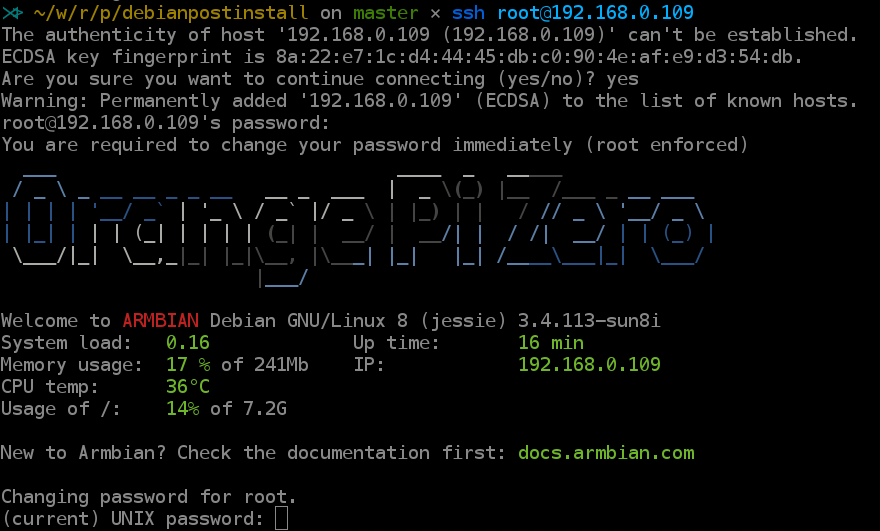
\includegraphics{src/img/OrangePiZero_FirstLogin.png}
\caption{Primer login en \emph{Orange Pi}}
\end{figure}

Lo primero es poner al dia el sistema:

\begin{verbatim}
apt-get update
apt-get upgrade
\end{verbatim}

Si quieres puedes reconfigurar el \emph{time zone}:

\begin{verbatim}
dpgk-reconfigura tzdata
\end{verbatim}

\subsubsection{Conexión WIFI}\label{conexiuxf3n-wifi}

Vamos a comprobar que todo va bien:

\begin{verbatim}
root@orangepizero:~# iwconfig
lo        no wireless extensions.

tunl0     no wireless extensions.

wlan0     IEEE 802.11bgn  ESSID:off/any
          Mode:Managed  Access Point: Not-Associated   Tx-Power=20 dBm
          Retry  long limit:7   RTS thr:off   Fragment thr:off
          Encryption key:off
          Power Management:on

eth0      no wireless extensions.
\end{verbatim}

Todo tiene buena pinta, vamos a ver si detecta WIFIs:

\begin{verbatim}
root@orangepizero:~# iwlist wlan0  scan |grep ESSID
                    ESSID:"wificlientesR"
                    ESSID:"casa_de_verano"
                    ESSID:"MOVISTAR_BEEF"
                    ESSID:"wificlientesR"
                    ESSID:"R-wlan90"
                    ESSID:"MOVISTAR_BAAF"
                    ESSID:"ababab"
                    ESSID:"WLAN 77"
                    ESSID:"castillo"
                    ESSID:"unaWifi"
                    ESSID:""
                    ESSID:"mikasa"
\end{verbatim}

Para configurar el wifi echamos un ojo al fichero
\texttt{/etc/network/interfaces} pero en ese mismo fichero encontramos
el aviso:

\begin{verbatim}
# Armbian ships with network-manager installed by default. To save you time
# and hassles consider using 'sudo nmtui' instead of configuring Wi-Fi settings
# manually.
\end{verbatim}

Así que basta con ejecutar \texttt{sudo\ nwtui} y ya podemos dar de alta
nuestra wifi (yo la prefiero con IP estática).

\begin{figure}[htbp]
\centering
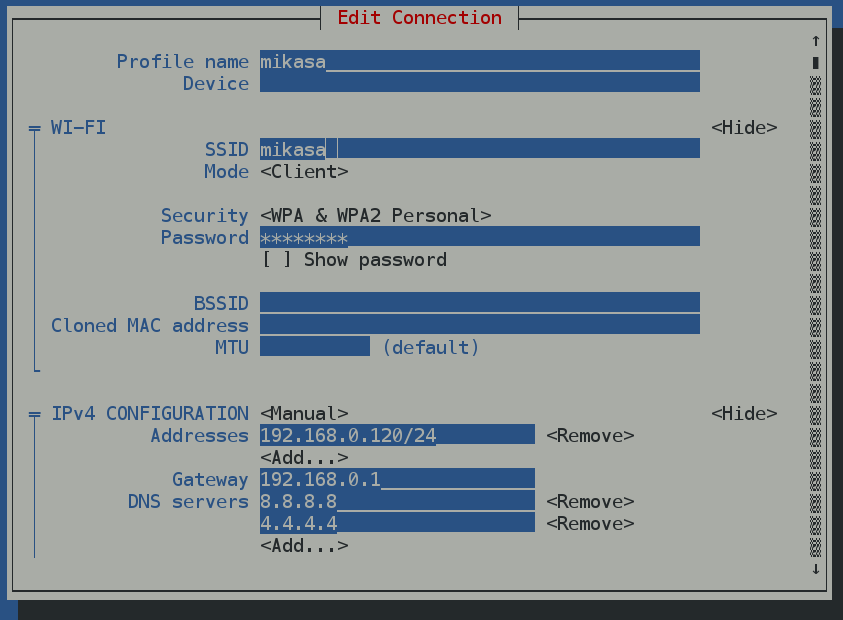
\includegraphics{src/img/OrangePiZero_tmtui.png}
\caption{Configuración WIFI}
\end{figure}

Ejecutamos \texttt{ifconfig} y ya vemos nuestro nuevo interface
configurado:

\begin{verbatim}
ifconfig

wlan0     Link encap:Ethernet  HWaddr a4:7c:f2:9a:97:7c
          inet addr:192.168.0.120  Bcast:192.168.0.255  Mask:255.255.255.0
          inet6 addr: fe80::a67c:f2ff:fe9a:977c/64 Scope:Link
          UP BROADCAST RUNNING MULTICAST  MTU:1500  Metric:1
          RX packets:2 errors:0 dropped:0 overruns:0 frame:0
          TX packets:8 errors:0 dropped:0 overruns:0 carrier:0
          collisions:0 txqueuelen:1000
          RX bytes:328 (328.0 B)  TX bytes:852 (852.0 B)
\end{verbatim}

\subsubsection{Referencias}\label{referencias-1}

\begin{itemize}
\tightlist
\item
  \href{http://www.orangepi.org/}{Página oficial}
\item
  \href{http://www.orangepi.org/downloadresources/}{Recursos oficiales}
  aquí hay imágenes y los esquemáticos
\item
  \href{https://www.aliexpress.com/store/1553371?spm=2114.8147860.0.0.F1q43C}{Tienda
  en Aliexpress}
\item
  \url{http://linux-sunxi.org/Bootable_SD_card}
\item
  \url{https://www.armbian.com/orange-pi-zero/}
\item
  \url{https://docs.armbian.com/User-Guide_Getting-Started/}
\item
  \url{https://docs.armbian.com/Hardware_Allwinner/}
\item
  \href{https://linux-sunxi.org/GPIO}{GPIO} Una explicación de como
  acceder al gpio desde terminal
\item
  \href{https://linux-sunxi.org/Orange_Pi_Zero}{Info variada} Aquí
  tenemos el esquema de pines
\end{itemize}

\subsection{Raspberry Pi Media Center}\label{raspberry-pi-media-center}

Bajamos la imagen con nuestro cliente torrent favorito desde
\href{https://github.com/aikoncwd/aikoncwd-rpi-mediacenter}{aquí}, no os
molesteis en clonar el directorio, hay que bajarse la imagen.

\begin{verbatim}
sudo dd if=./Mediacenter-AikonCWD-v6.img  of=/dev/mmcblk0 bs=4M
\end{verbatim}

Arrancamos con la toma ethernet conectada al router y nos conectamos
tras averigurar la IP con \texttt{nmap} (ver \emph{Orange Pi Zero})

\begin{figure}[htbp]
\centering
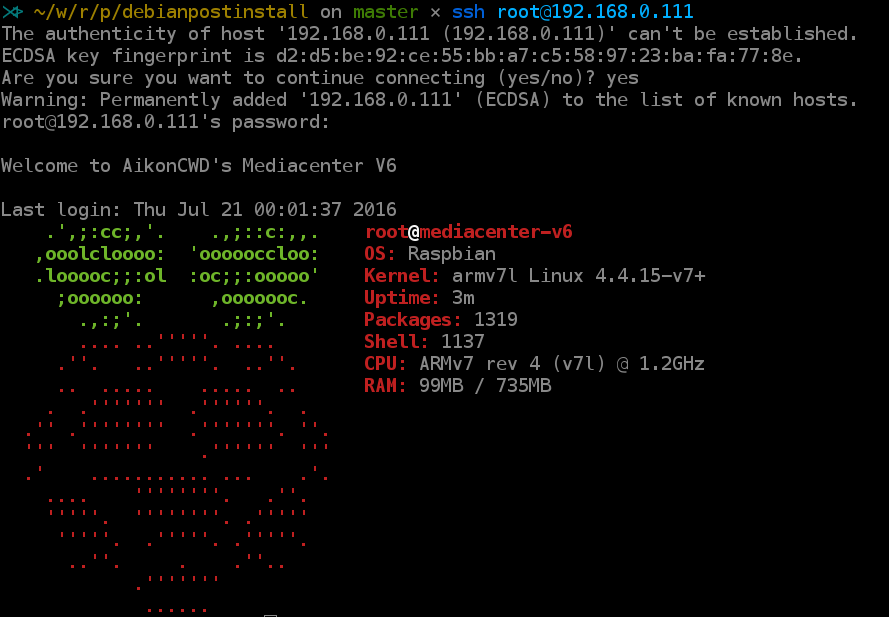
\includegraphics{src/img/RaspiFirstLogin.png}
\caption{Primer login en Raspberry}
\end{figure}

Una vez instalado los pasos recomendados:

\begin{enumerate}
\def\labelenumi{\arabic{enumi}.}
\item
  Cambiar la password de root: \texttt{passwd}
\item
  Fijar una IP estática: Editamos el fichero \texttt{/etc/dhcpcd.conf},
  ya de paso configuramos la IP estática para la WIFI

\begin{verbatim}
interface eth0
static ip_address=192.168.0.125/24
static routers=192.168.0.1
static domain_name_servers=8.8.8.8

interface wlan0
static ip_address=192.168.0.126/24
static routers=192.168.0.1
static domain_name_servers=8.8.8.8
\end{verbatim}

  Una vez cambiado el fichero hay que reiniciar con
  \texttt{shutdown\ -r\ now}
\item
  Configurar la WIFI, en esta parte damos por supuesto que tenemos la
  wifi con WPA activado.

  Echamos un ojo a nuestro interfaz radio con \texttt{iwconfig}, si
  aparece el \texttt{wlan0} todo va bien.

\begin{verbatim}
wlan0     IEEE 802.11bgn  ESSID:off/any
          Mode:Managed  Access Point: Not-Associated   Tx-Power=31 dBm
          Retry short limit:7   RTS thr:off   Fragment thr:off
          Encryption key:off
          Power Management:on
\end{verbatim}

  Tenemos que editar el fichero \texttt{/etc/network/interfaces} y
  asegurarnos de tener el \texttt{wlan0} como sigue:

\begin{verbatim}
allow-hotplug wlan0
iface wlan0 inet manual
    wpa-conf /etc/wpa_supplicant/wpa_supplicant.conf
\end{verbatim}

  Ahora vamos a editar el fichero de configuración de
  \texttt{wpa\_supplicant}, es decir
  \texttt{/etc/wpa\_supplicant/wpa\_supplicant.conf} y añadir un bloque
  \texttt{network} que sea como el que va a continuación, de paso he
  cambiado el \texttt{country} a ``ES'', asi que queda así:

\begin{verbatim}
country=ES
ctrl_interface=DIR=/var/run/wpa_supplicant GROUP=netdev
update_config=1
network={
  ssid="YOURSSID"
  psk="YOURPASSWORD"
}
\end{verbatim}

  Un reinicio y listos: \texttt{shutdown\ -r\ now}
\end{enumerate}

\subsection{Grabar time-lapse del
escritorio}\label{grabar-time-lapse-del-escritorio}

\subsubsection{Usando avconv}\label{usando-avconv}

Capturas periódicas de la pantalla:

\begin{verbatim}
avconv -video_size 1366x768 -framerate 1/10 -f x11grab -i :0.0+0,0 -pix_fmt rgb24 ~/tmp/frames/frame_%05d.png
\end{verbatim}

El framerate son imágenes por segundo, así que aquí estamos diciendo que
capturamos una imagen cada 10 sg.

\section{TODO}\label{todo-1}

\begin{itemize}
\tightlist
\item
  cinelerra
\item
  playonlinux
\item
  krita
\item
  mypaint
\item
  qStopmotion
\item
  chibios

  \begin{itemize}
  \tightlist
  \item
    {[}http://wiki.chibios.org/dokuwiki/doku.php?id=chibios:community:setup:openocd\_chibios{]}
  \item
    {[}http://www.josho.org/blog/blog/2014/11/30/nucleo-gcc/{]}
  \item
    {[}http://www.stevebate.net/chibios-rpi/GettingStarted.html{]}
  \end{itemize}
\item
  ICE Studio
\item
  Inkscape

  \begin{itemize}
  \tightlist
  \item
    \url{https://elizsarobhasa.makes.org/thimble/MTMwNDIzMjE5Mg==/3d-printing-from-a-2d-drawing}
  \item
    Instalar tb jessyink
  \end{itemize}
\item
  rclone \url{https://syncthing.net/}
\item
  vmware (no creo, virtualbox va genial)
\item
  Astronomía
\end{itemize}

\section{Links}\label{links}

\begin{itemize}
\tightlist
\item
  \href{https://wiki.debian.org/systemd}{Systemd}
\item
  \href{https://wiki.gnome.org/Design/OS/KeyboardShortcuts}{Gnome
  shortcuts}
\item
  \href{https://www.linux.com/learn/easy-steps-make-gnome-3-more-efficient}{Gnome
  optimizaciones}
\item
  \href{https://diversidadyunpocodetodo.blogspot.com.es/2015/03/sensores-temperatura-hardware-discos-cpu-debian-ubuntu.html}{Instalación
  Debian}
\item
  \href{http://joshldavis.com/2014/07/26/oh-my-zsh-is-a-disease-antigen-is-the-vaccine/}{zsh}
\item
  \href{http://blog.namangoel.com/zsh-with-antigen}{zsh}
\item
  \url{https://www.roaringpenguin.com/products/remind}
\item
  \url{http://taskwarrior.org/}
\end{itemize}

\section{Licencia}\label{licencia}

\begin{verbatim}

Attribution-ShareAlike 4.0 International

=======================================================================

Creative Commons Corporation ("Creative Commons") is not a law firm and
does not provide legal services or legal advice. Distribution of
Creative Commons public licenses does not create a lawyer-client or
other relationship. Creative Commons makes its licenses and related
information available on an "as-is" basis. Creative Commons gives no
warranties regarding its licenses, any material licensed under their
terms and conditions, or any related information. Creative Commons
disclaims all liability for damages resulting from their use to the
fullest extent possible.

Using Creative Commons Public Licenses

Creative Commons public licenses provide a standard set of terms and
conditions that creators and other rights holders may use to share
original works of authorship and other material subject to copyright
and certain other rights specified in the public license below. The
following considerations are for informational purposes only, are not
exhaustive, and do not form part of our licenses.

     Considerations for licensors: Our public licenses are
     intended for use by those authorized to give the public
     permission to use material in ways otherwise restricted by
     copyright and certain other rights. Our licenses are
     irrevocable. Licensors should read and understand the terms
     and conditions of the license they choose before applying it.
     Licensors should also secure all rights necessary before
     applying our licenses so that the public can reuse the
     material as expected. Licensors should clearly mark any
     material not subject to the license. This includes other CC-
     licensed material, or material used under an exception or
     limitation to copyright. More considerations for licensors:
    wiki.creativecommons.org/Considerations_for_licensors

     Considerations for the public: By using one of our public
     licenses, a licensor grants the public permission to use the
     licensed material under specified terms and conditions. If
     the licensor's permission is not necessary for any reason--for
     example, because of any applicable exception or limitation to
     copyright--then that use is not regulated by the license. Our
     licenses grant only permissions under copyright and certain
     other rights that a licensor has authority to grant. Use of
     the licensed material may still be restricted for other
     reasons, including because others have copyright or other
     rights in the material. A licensor may make special requests,
     such as asking that all changes be marked or described.
     Although not required by our licenses, you are encouraged to
     respect those requests where reasonable. More_considerations
     for the public:
    wiki.creativecommons.org/Considerations_for_licensees

=======================================================================

Creative Commons Attribution-ShareAlike 4.0 International Public
License

By exercising the Licensed Rights (defined below), You accept and agree
to be bound by the terms and conditions of this Creative Commons
Attribution-ShareAlike 4.0 International Public License ("Public
License"). To the extent this Public License may be interpreted as a
contract, You are granted the Licensed Rights in consideration of Your
acceptance of these terms and conditions, and the Licensor grants You
such rights in consideration of benefits the Licensor receives from
making the Licensed Material available under these terms and
conditions.


Section 1 -- Definitions.

  a. Adapted Material means material subject to Copyright and Similar
     Rights that is derived from or based upon the Licensed Material
     and in which the Licensed Material is translated, altered,
     arranged, transformed, or otherwise modified in a manner requiring
     permission under the Copyright and Similar Rights held by the
     Licensor. For purposes of this Public License, where the Licensed
     Material is a musical work, performance, or sound recording,
     Adapted Material is always produced where the Licensed Material is
     synched in timed relation with a moving image.

  b. Adapter's License means the license You apply to Your Copyright
     and Similar Rights in Your contributions to Adapted Material in
     accordance with the terms and conditions of this Public License.

  c. BY-SA Compatible License means a license listed at
     creativecommons.org/compatiblelicenses, approved by Creative
     Commons as essentially the equivalent of this Public License.

  d. Copyright and Similar Rights means copyright and/or similar rights
     closely related to copyright including, without limitation,
     performance, broadcast, sound recording, and Sui Generis Database
     Rights, without regard to how the rights are labeled or
     categorized. For purposes of this Public License, the rights
     specified in Section 2(b)(1)-(2) are not Copyright and Similar
     Rights.

  e. Effective Technological Measures means those measures that, in the
     absence of proper authority, may not be circumvented under laws
     fulfilling obligations under Article 11 of the WIPO Copyright
     Treaty adopted on December 20, 1996, and/or similar international
     agreements.

  f. Exceptions and Limitations means fair use, fair dealing, and/or
     any other exception or limitation to Copyright and Similar Rights
     that applies to Your use of the Licensed Material.

  g. License Elements means the license attributes listed in the name
     of a Creative Commons Public License. The License Elements of this
     Public License are Attribution and ShareAlike.

  h. Licensed Material means the artistic or literary work, database,
     or other material to which the Licensor applied this Public
     License.

  i. Licensed Rights means the rights granted to You subject to the
     terms and conditions of this Public License, which are limited to
     all Copyright and Similar Rights that apply to Your use of the
     Licensed Material and that the Licensor has authority to license.

  j. Licensor means the individual(s) or entity(ies) granting rights
     under this Public License.

  k. Share means to provide material to the public by any means or
     process that requires permission under the Licensed Rights, such
     as reproduction, public display, public performance, distribution,
     dissemination, communication, or importation, and to make material
     available to the public including in ways that members of the
     public may access the material from a place and at a time
     individually chosen by them.

  l. Sui Generis Database Rights means rights other than copyright
     resulting from Directive 96/9/EC of the European Parliament and of
     the Council of 11 March 1996 on the legal protection of databases,
     as amended and/or succeeded, as well as other essentially
     equivalent rights anywhere in the world.

  m. You means the individual or entity exercising the Licensed Rights
     under this Public License. Your has a corresponding meaning.


Section 2 -- Scope.

  a. License grant.

       1. Subject to the terms and conditions of this Public License,
          the Licensor hereby grants You a worldwide, royalty-free,
          non-sublicensable, non-exclusive, irrevocable license to
          exercise the Licensed Rights in the Licensed Material to:

            a. reproduce and Share the Licensed Material, in whole or
               in part; and

            b. produce, reproduce, and Share Adapted Material.

       2. Exceptions and Limitations. For the avoidance of doubt, where
          Exceptions and Limitations apply to Your use, this Public
          License does not apply, and You do not need to comply with
          its terms and conditions.

       3. Term. The term of this Public License is specified in Section
          6(a).

       4. Media and formats; technical modifications allowed. The
          Licensor authorizes You to exercise the Licensed Rights in
          all media and formats whether now known or hereafter created,
          and to make technical modifications necessary to do so. The
          Licensor waives and/or agrees not to assert any right or
          authority to forbid You from making technical modifications
          necessary to exercise the Licensed Rights, including
          technical modifications necessary to circumvent Effective
          Technological Measures. For purposes of this Public License,
          simply making modifications authorized by this Section 2(a)
          (4) never produces Adapted Material.

       5. Downstream recipients.

            a. Offer from the Licensor -- Licensed Material. Every
               recipient of the Licensed Material automatically
               receives an offer from the Licensor to exercise the
               Licensed Rights under the terms and conditions of this
               Public License.

            b. Additional offer from the Licensor -- Adapted Material.
               Every recipient of Adapted Material from You
               automatically receives an offer from the Licensor to
               exercise the Licensed Rights in the Adapted Material
               under the conditions of the Adapter's License You apply.

            c. No downstream restrictions. You may not offer or impose
               any additional or different terms or conditions on, or
               apply any Effective Technological Measures to, the
               Licensed Material if doing so restricts exercise of the
               Licensed Rights by any recipient of the Licensed
               Material.

       6. No endorsement. Nothing in this Public License constitutes or
          may be construed as permission to assert or imply that You
          are, or that Your use of the Licensed Material is, connected
          with, or sponsored, endorsed, or granted official status by,
          the Licensor or others designated to receive attribution as
          provided in Section 3(a)(1)(A)(i).

  b. Other rights.

       1. Moral rights, such as the right of integrity, are not
          licensed under this Public License, nor are publicity,
          privacy, and/or other similar personality rights; however, to
          the extent possible, the Licensor waives and/or agrees not to
          assert any such rights held by the Licensor to the limited
          extent necessary to allow You to exercise the Licensed
          Rights, but not otherwise.

       2. Patent and trademark rights are not licensed under this
          Public License.

       3. To the extent possible, the Licensor waives any right to
          collect royalties from You for the exercise of the Licensed
          Rights, whether directly or through a collecting society
          under any voluntary or waivable statutory or compulsory
          licensing scheme. In all other cases the Licensor expressly
          reserves any right to collect such royalties.


Section 3 -- License Conditions.

Your exercise of the Licensed Rights is expressly made subject to the
following conditions.

  a. Attribution.

       1. If You Share the Licensed Material (including in modified
          form), You must:

            a. retain the following if it is supplied by the Licensor
               with the Licensed Material:

                 i. identification of the creator(s) of the Licensed
                    Material and any others designated to receive
                    attribution, in any reasonable manner requested by
                    the Licensor (including by pseudonym if
                    designated);

                ii. a copyright notice;

               iii. a notice that refers to this Public License;

                iv. a notice that refers to the disclaimer of
                    warranties;

                 v. a URI or hyperlink to the Licensed Material to the
                    extent reasonably practicable;

            b. indicate if You modified the Licensed Material and
               retain an indication of any previous modifications; and

            c. indicate the Licensed Material is licensed under this
               Public License, and include the text of, or the URI or
               hyperlink to, this Public License.

       2. You may satisfy the conditions in Section 3(a)(1) in any
          reasonable manner based on the medium, means, and context in
          which You Share the Licensed Material. For example, it may be
          reasonable to satisfy the conditions by providing a URI or
          hyperlink to a resource that includes the required
          information.

       3. If requested by the Licensor, You must remove any of the
          information required by Section 3(a)(1)(A) to the extent
          reasonably practicable.

  b. ShareAlike.

     In addition to the conditions in Section 3(a), if You Share
     Adapted Material You produce, the following conditions also apply.

       1. The Adapter's License You apply must be a Creative Commons
          license with the same License Elements, this version or
          later, or a BY-SA Compatible License.

       2. You must include the text of, or the URI or hyperlink to, the
          Adapter's License You apply. You may satisfy this condition
          in any reasonable manner based on the medium, means, and
          context in which You Share Adapted Material.

       3. You may not offer or impose any additional or different terms
          or conditions on, or apply any Effective Technological
          Measures to, Adapted Material that restrict exercise of the
          rights granted under the Adapter's License You apply.


Section 4 -- Sui Generis Database Rights.

Where the Licensed Rights include Sui Generis Database Rights that
apply to Your use of the Licensed Material:

  a. for the avoidance of doubt, Section 2(a)(1) grants You the right
     to extract, reuse, reproduce, and Share all or a substantial
     portion of the contents of the database;

  b. if You include all or a substantial portion of the database
     contents in a database in which You have Sui Generis Database
     Rights, then the database in which You have Sui Generis Database
     Rights (but not its individual contents) is Adapted Material,

     including for purposes of Section 3(b); and
  c. You must comply with the conditions in Section 3(a) if You Share
     all or a substantial portion of the contents of the database.

For the avoidance of doubt, this Section 4 supplements and does not
replace Your obligations under this Public License where the Licensed
Rights include other Copyright and Similar Rights.


Section 5 -- Disclaimer of Warranties and Limitation of Liability.

  a. UNLESS OTHERWISE SEPARATELY UNDERTAKEN BY THE LICENSOR, TO THE
     EXTENT POSSIBLE, THE LICENSOR OFFERS THE LICENSED MATERIAL AS-IS
     AND AS-AVAILABLE, AND MAKES NO REPRESENTATIONS OR WARRANTIES OF
     ANY KIND CONCERNING THE LICENSED MATERIAL, WHETHER EXPRESS,
     IMPLIED, STATUTORY, OR OTHER. THIS INCLUDES, WITHOUT LIMITATION,
     WARRANTIES OF TITLE, MERCHANTABILITY, FITNESS FOR A PARTICULAR
     PURPOSE, NON-INFRINGEMENT, ABSENCE OF LATENT OR OTHER DEFECTS,
     ACCURACY, OR THE PRESENCE OR ABSENCE OF ERRORS, WHETHER OR NOT
     KNOWN OR DISCOVERABLE. WHERE DISCLAIMERS OF WARRANTIES ARE NOT
     ALLOWED IN FULL OR IN PART, THIS DISCLAIMER MAY NOT APPLY TO YOU.

  b. TO THE EXTENT POSSIBLE, IN NO EVENT WILL THE LICENSOR BE LIABLE
     TO YOU ON ANY LEGAL THEORY (INCLUDING, WITHOUT LIMITATION,
     NEGLIGENCE) OR OTHERWISE FOR ANY DIRECT, SPECIAL, INDIRECT,
     INCIDENTAL, CONSEQUENTIAL, PUNITIVE, EXEMPLARY, OR OTHER LOSSES,
     COSTS, EXPENSES, OR DAMAGES ARISING OUT OF THIS PUBLIC LICENSE OR
     USE OF THE LICENSED MATERIAL, EVEN IF THE LICENSOR HAS BEEN
     ADVISED OF THE POSSIBILITY OF SUCH LOSSES, COSTS, EXPENSES, OR
     DAMAGES. WHERE A LIMITATION OF LIABILITY IS NOT ALLOWED IN FULL OR
     IN PART, THIS LIMITATION MAY NOT APPLY TO YOU.

  c. The disclaimer of warranties and limitation of liability provided
     above shall be interpreted in a manner that, to the extent
     possible, most closely approximates an absolute disclaimer and
     waiver of all liability.


Section 6 -- Term and Termination.

  a. This Public License applies for the term of the Copyright and
     Similar Rights licensed here. However, if You fail to comply with
     this Public License, then Your rights under this Public License
     terminate automatically.

  b. Where Your right to use the Licensed Material has terminated under
     Section 6(a), it reinstates:

       1. automatically as of the date the violation is cured, provided
          it is cured within 30 days of Your discovery of the
          violation; or

       2. upon express reinstatement by the Licensor.

     For the avoidance of doubt, this Section 6(b) does not affect any
     right the Licensor may have to seek remedies for Your violations
     of this Public License.

  c. For the avoidance of doubt, the Licensor may also offer the
     Licensed Material under separate terms or conditions or stop
     distributing the Licensed Material at any time; however, doing so
     will not terminate this Public License.

  d. Sections 1, 5, 6, 7, and 8 survive termination of this Public
     License.


Section 7 -- Other Terms and Conditions.

  a. The Licensor shall not be bound by any additional or different
     terms or conditions communicated by You unless expressly agreed.

  b. Any arrangements, understandings, or agreements regarding the
     Licensed Material not stated herein are separate from and
     independent of the terms and conditions of this Public License.


Section 8 -- Interpretation.

  a. For the avoidance of doubt, this Public License does not, and
     shall not be interpreted to, reduce, limit, restrict, or impose
     conditions on any use of the Licensed Material that could lawfully
     be made without permission under this Public License.

  b. To the extent possible, if any provision of this Public License is
     deemed unenforceable, it shall be automatically reformed to the
     minimum extent necessary to make it enforceable. If the provision
     cannot be reformed, it shall be severed from this Public License
     without affecting the enforceability of the remaining terms and
     conditions.

  c. No term or condition of this Public License will be waived and no
     failure to comply consented to unless expressly agreed to by the
     Licensor.

  d. Nothing in this Public License constitutes or may be interpreted
     as a limitation upon, or waiver of, any privileges and immunities
     that apply to the Licensor or You, including from the legal
     processes of any jurisdiction or authority.


=======================================================================

Creative Commons is not a party to its public
licenses. Notwithstanding, Creative Commons may elect to apply one of
its public licenses to material it publishes and in those instances
will be considered the “Licensor.” The text of the Creative Commons
public licenses is dedicated to the public domain under the CC0 Public
Domain Dedication. Except for the limited purpose of indicating that
material is shared under a Creative Commons public license or as
otherwise permitted by the Creative Commons policies published at
creativecommons.org/policies, Creative Commons does not authorize the
use of the trademark "Creative Commons" or any other trademark or logo
of Creative Commons without its prior written consent including,
without limitation, in connection with any unauthorized modifications
to any of its public licenses or any other arrangements,
understandings, or agreements concerning use of licensed material. For
the avoidance of doubt, this paragraph does not form part of the
public licenses.

Creative Commons may be contacted at creativecommons.org.
\end{verbatim}

\end{document}
